%% LyX 2.3.4.2 created this file.  For more info, see http://www.lyx.org/.
%% Do not edit unless you really know what you are doing.
\documentclass[english,dvipsnames,aspectratio=169,handout]{beamer}
\usepackage{mathptmx}
\usepackage{eulervm}
\usepackage[T1]{fontenc}
\usepackage[latin9]{inputenc}
\usepackage{babel}
\usepackage{amstext}
\usepackage{amssymb}
\usepackage{graphicx}
\usepackage{ifthen}
\usepackage{xcolor}
\usepackage{xspace}
\usepackage{booktabs}
\usepackage{xpatch}
\usepackage{multirow}
\usepackage{colortbl}
\usepackage{pgfpages}
\usepackage{tikz}
\usetikzlibrary{tikzmark}
\usetikzlibrary{calc}
\usetikzlibrary{positioning}
\usepackage{pgfplots}
%\pgfplotsset{compat=1.17}
\usepackage{booktabs}



\xpatchcmd{\itemize}
  {\def\makelabel}
  {\ifnum\@itemdepth=1\relax
     \setlength\itemsep{2ex}% separation for first level
   \else
     \ifnum\@itemdepth=2\relax
       \setlength\itemsep{1ex}% separation for second level
     \else
       \ifnum\@itemdepth=3\relax
         \setlength\itemsep{0.5ex}% separation for third level
   \fi\fi\fi\def\makelabel
  }
 {}
 {}

\ifx\hypersetup\undefined
  \AtBeginDocument{%
    \hypersetup{unicode=true,pdfusetitle,
 bookmarks=true,bookmarksnumbered=false,bookmarksopen=false,
 breaklinks=false,pdfborder={0 0 0},pdfborderstyle={},backref=false,colorlinks=true,
 allcolors=NYUPurple,urlcolor=LightPurple}
  }
\else
  \hypersetup{unicode=true,pdfusetitle,
 bookmarks=true,bookmarksnumbered=false,bookmarksopen=false,
 breaklinks=false,pdfborder={0 0 0},pdfborderstyle={},backref=false,colorlinks=true,
 allcolors=NYUPurple,urlcolor=LightPurple}
\fi

\makeatletter

%%%%%%%%%%%%%%%%%%%%%%%%%%%%%% LyX specific LaTeX commands.
%% Because html converters don't know tabularnewline
\providecommand{\tabularnewline}{\\}

%%%%%%%%%%%%%%%%%%%%%%%%%%%%%% Textclass specific LaTeX commands.
% this default might be overridden by plain title style
\newcommand\makebeamertitle{\frame{\maketitle}}%
% (ERT) argument for the TOC
\AtBeginDocument{%
  \let\origtableofcontents=\tableofcontents
  \def\tableofcontents{\@ifnextchar[{\origtableofcontents}{\gobbletableofcontents}}
  \def\gobbletableofcontents#1{\origtableofcontents}
}

%%%%%%%%%%%%%%%%%%%%%%%%%%%%%% User specified LaTeX commands.
\usetheme{CambridgeUS} 
\beamertemplatenavigationsymbolsempty


% Set Color ==============================
\definecolor{NYUPurple}{RGB}{87,6,140}
\definecolor{LightPurple}{RGB}{165,11,255}


\setbeamercolor{title}{fg=NYUPurple}
\setbeamercolor{frametitle}{fg=NYUPurple}

\setbeamercolor{background canvas}{fg=NYUPurple, bg=white}
\setbeamercolor{background}{fg=black, bg=NYUPurple}

\setbeamercolor{palette primary}{fg=black, bg=gray!30!white}
\setbeamercolor{palette secondary}{fg=black, bg=gray!20!white}
\setbeamercolor{palette tertiary}{fg=gray!20!white, bg=NYUPurple}

\setbeamertemplate{headline}{}
\setbeamerfont{itemize/enumerate body}{}
\setbeamerfont{itemize/enumerate subbody}{size=\normalsize}

\setbeamercolor{parttitle}{fg=NYUPurple}
\setbeamercolor{sectiontitle}{fg=NYUPurple}
\setbeamercolor{sectionname}{fg=NYUPurple}
\setbeamercolor{section page}{fg=NYUPurple}
%\setbeamercolor{description item}{fg=NYUPurple}
%\setbeamercolor{block title}{fg=NYUPurple}

\setbeamertemplate{blocks}[rounded][shadow=false]
\setbeamercolor{block body}{bg=normal text.bg!90!NYUPurple}
\setbeamercolor{block title}{bg=NYUPurple!30, fg=NYUPurple}



\AtBeginSection[]{
  \begin{frame}
  \vfill
  \centering
\setbeamercolor{section title}{fg=NYUPurple}
 \begin{beamercolorbox}[sep=8pt,center,shadow=true,rounded=true]{title}
    \usebeamerfont{title}\usebeamercolor[fg]{title}\insertsectionhead\par%
  \end{beamercolorbox}
  \vfill
  \end{frame}
}

\makeatother

\setlength{\parskip}{\medskipamount} 

\input ../macros

\begin{document}
\input ../rosenberg-macros

%\setbeameroption{show notes on second screen}

\title[DS-GA 1003]{Backpropagation}
\author{He He}
\date{April 20, 2021}
\institute{CDS, NYU}

\makebeamertitle
\mode<article>{Just in article version}

\section{Back-propagation}
\begin{frame}
{A brief history of artificial neural networks}
\begin{simpleblock}{early 1940s--late 1960s}
\begin{itemize}
\item Initial idea from neuroscience: create a computational model of neural networks.
\item Development: perceptron [Rosenblatt, 1958], networks with many layers.
\item Optimization: automatic differentiation [Linnainmaa, 1970].
\end{itemize}
\end{simpleblock}
\pause

\begin{simpleblock}{late 1960s--late 1980s}
\begin{itemize}
\item Computers didn't have enough processing power [Minsky and Papert, 1969].
\item Back-propagation invented [Werbos, 1975] (but still hard to train).
\item AI research focused on expert systems and symbolic systems.
\end{itemize}
\end{simpleblock}
\pause

\begin{simpleblock}{late 1980s--early 2000s}
\begin{itemize}
\item SVMs and linear models dominated ML.
\item Continual developments in ANN: Schmidhuber, Hinton, Lecun etc.
\end{itemize}
\end{simpleblock}
\note[item]{The initial idea of an ANN started from neuroscience, but the model is not to be confused with the thing in our brain. There's very little connection, if anything at all. In the 50's and 60's, the idea got developed and NN with multiple layers were designed.}
\note[item]{For a long time, no one knows how to train it. The Minsky and Papert paper pointed out that computers at that time aren't powerful enough. In 1975, backpropagation was invented, but there are still many problem in training these models, such as gradient vanishing.}
\note[item]{Until early 2000's, SVM and other linear models dominated ML. But the NN research was still going on and important development comes from groups led by S, H, Y etc. Around 2006, people find that with big data and compute, training doesn't seem to be an issue any more. You know the story afterwards.}
\note[item]{Next, let's go through the backpropagation algorithm.}
\end{frame}

\begin{frame}{Example: MLP Regression }
\begin{itemize}
\item \textbf{Input space}: $\cx=\reals$ 
\item \textbf{Action Space / Output space}: $\ca=\cy=\reals$
\item \textbf{Hypothesis space}: MLPs with a single 3-node hidden layer:
\[
f(x)=w_{0}+w_{1}h_{1}(x)+w_{2}h_{2}(x)+w_{3}h_{3}(x),
\]
where 
\[
h_{i}(x)=\sigma(v_{i}x+b_{i})\text{ for }i=1,2,3,
\]
for some fixed activation function $\sigma:\reals\to\reals$. 


\item What are the parameters we need to fit?
\[
\pause b_{1},b_{2},b_{3},v_{1},v_{2},v_{3},w_{0},w_{1},w_{2},w_{3}\in\reals
\]
\end{itemize}
\note[item]{How do we learn these parameters?}
\end{frame}
%
%
\begin{frame}{How to choose the best hypothesis?}
\begin{itemize}[<+->]
\item As usual, choose our prediction function using empirical risk minimization.
\item Our hypothesis space is parameterized by
\[
\theta=\left(b_{1},b_{2},b_{3},v_{1},v_{2},v_{3},w_{0},w_{1},w_{2},w_{3}\right)\in\Theta=\reals^{10}
\]
\item For a training set $(x_{1},y_{1}),\ldots,(x_{n},y_{n})$, find
\[
\hat{\theta}=\argmin_{\theta\in\reals^{10}}\frac{1}{n}\sum_{i=1}^{n}\left(f(x_{i}; \theta)-y_{i}\right)^{2}.
\]
\item Gradient descent:
\begin{itemize}
\item Is it differentiable w.r.t. $\theta$? $f(x) = {\color{blue}w_{0}}+\sum_{i=1}^{3}{\color{blue}w_{i}}\tanh({\color{blue}v_{i}}x+{\color{blue}b_{i}})$.
\item Is it convex in $\theta$? Might converge to a local minimum.
\end{itemize}
\end{itemize}
\end{frame}

\begin{frame}
{Gradient descent for (large) neural networks}
\begin{itemize}[<+->]
\item Mathematically, it's just \emph{partial derivatives}, which you can compute by hand using the \emph{chain rule}.
\begin{itemize}[<.->]
\item In practice, this could be \alarm{time-consuming} and \alarm{error-prone}.
\end{itemize}
\item How do we compute gradients in a systematic and efficient way?
\begin{itemize}[<.->]
\item \emph{Back-propagation} (a special case of automatic differentiation).
\item Not limited to neural networks.
\end{itemize}
\item Visualize with \emph{computation graphs}.
\begin{itemize}[<.->]
\item Avoid long equations.
\item Structure of the computation (\textcolor{Green}{modularity} and \textcolor{Green}{dependency}), which allows for modern computation frameworks such as Tensorflow/Pytorch/MXNet/etc.
\end{itemize}
\end{itemize}
\end{frame}

\subsection{Partial Derivatives and the Chain Rule}

\begin{frame}
{Function as a graph}
\begin{itemize}
\item Function as a \emph{node} that takes in a set of \emph{inputs} and produces a set of \emph{outputs}.
\item Example: $g:\reals^{p}\to\reals^{n}$.
\end{itemize}

\begin{columns}[t]
\column{.4\textwidth}
\begin{itemize}
\item Typical computation graph:
\end{itemize}
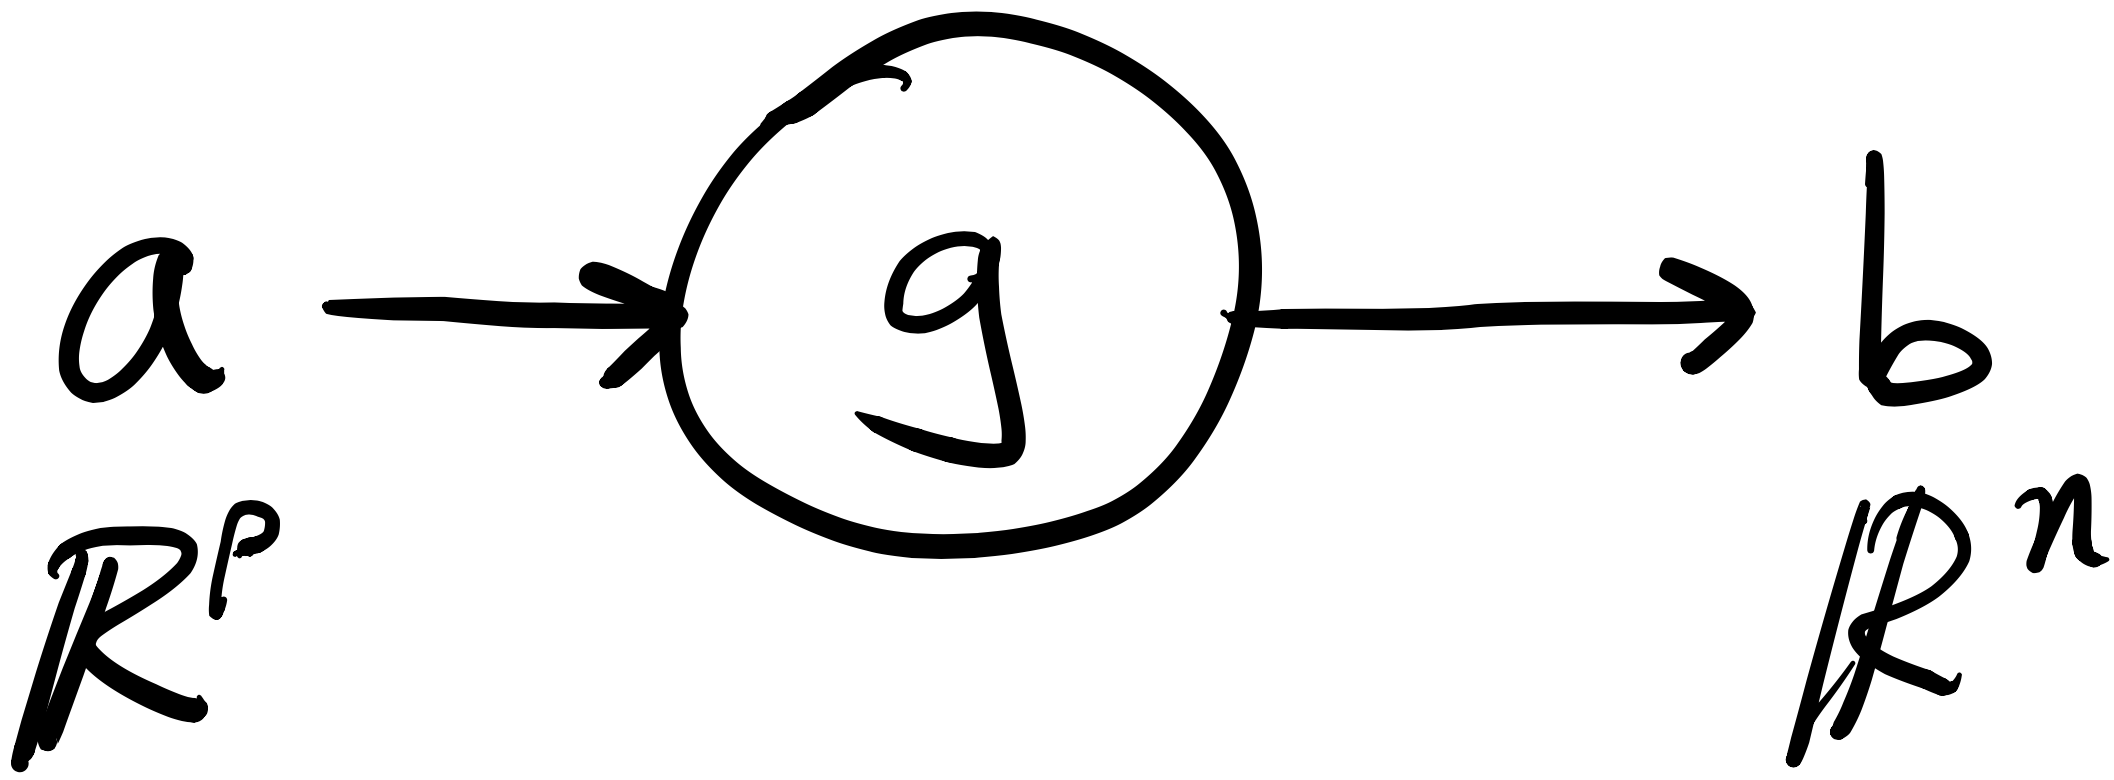
\includegraphics[scale=0.07]{figures/one-fn-comp-graph}

\pause{}

\column{.4\textwidth}
\begin{itemize}
\item Broken out into components:
\end{itemize}
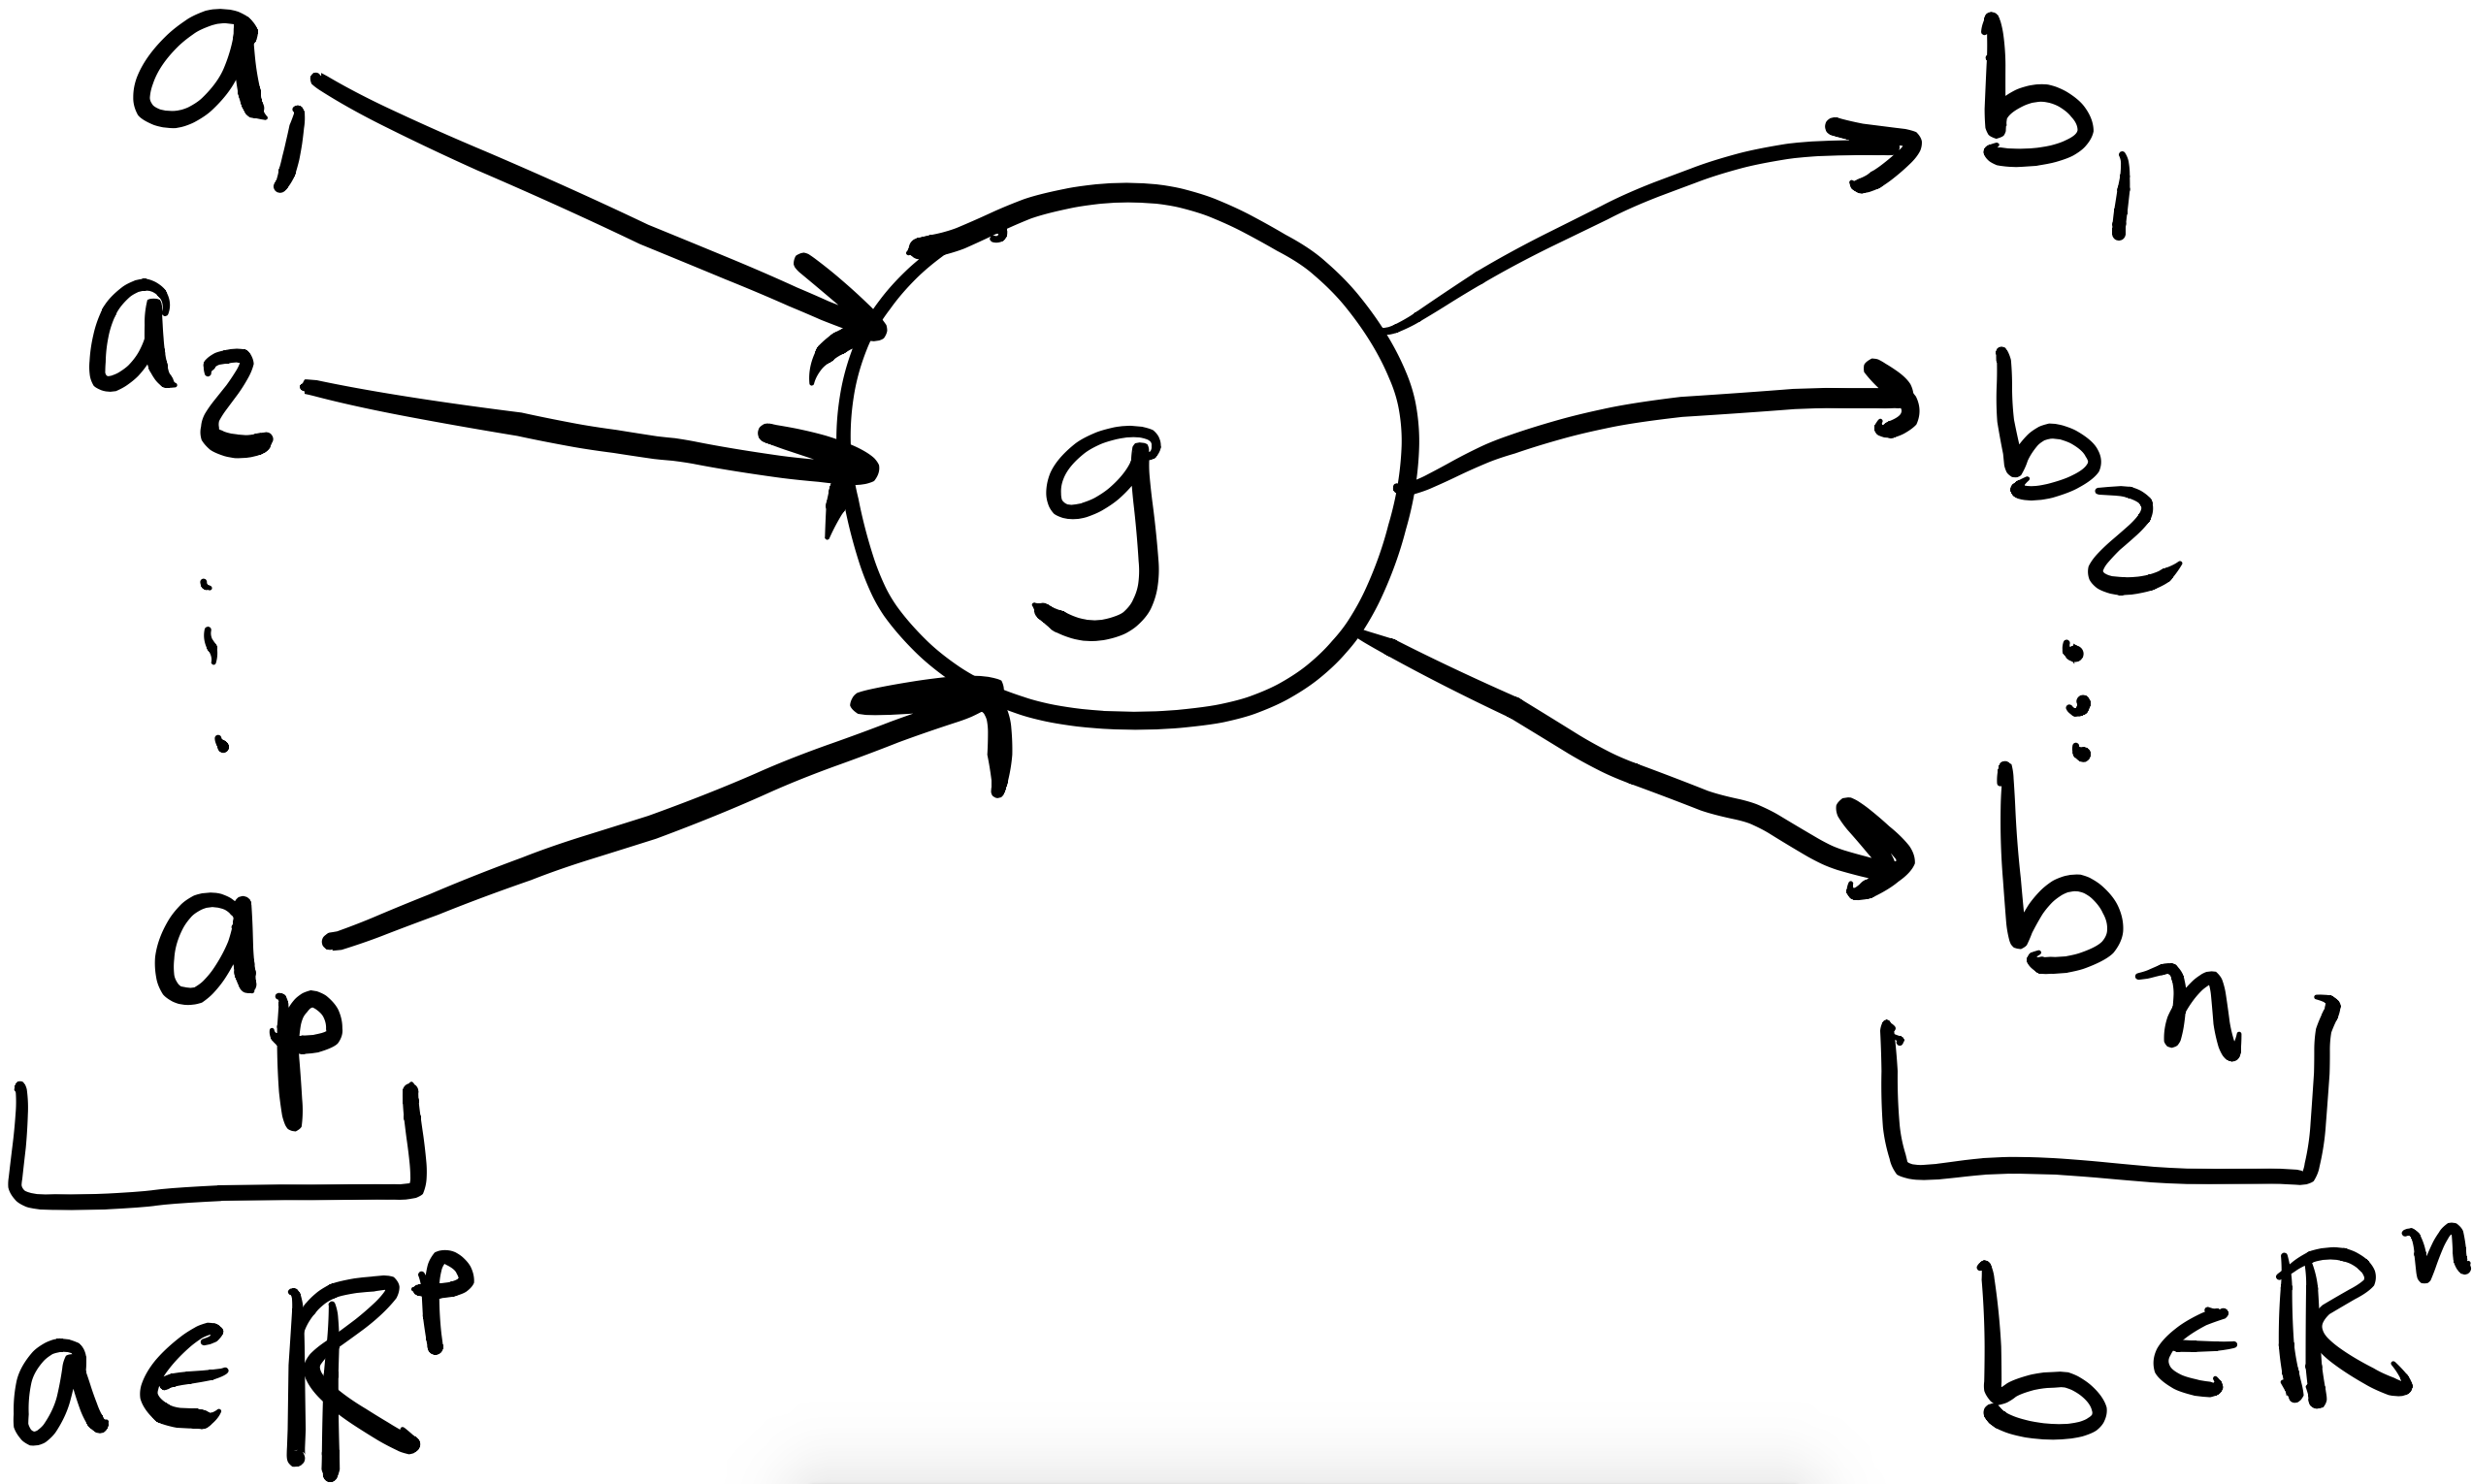
\includegraphics[scale=0.07]{figures/one-fn-comp-graph-partials}
\end{columns}
\note[item]{Conceptually, let's now think of functions as a graph. We have a node representing the computation happens in the function. The arrows or directed edges represent the input and output.}
\end{frame}

\begin{frame}{Partial Derivatives of an affine function}
\begin{itemize}
\item Define the affine function $g(x)=Mx+c$, for $M\in\reals^{n\times p}$
and $c\in\reals$.
\end{itemize}
\begin{columns}[t]

\column{.35\textwidth}
\begin{figure}
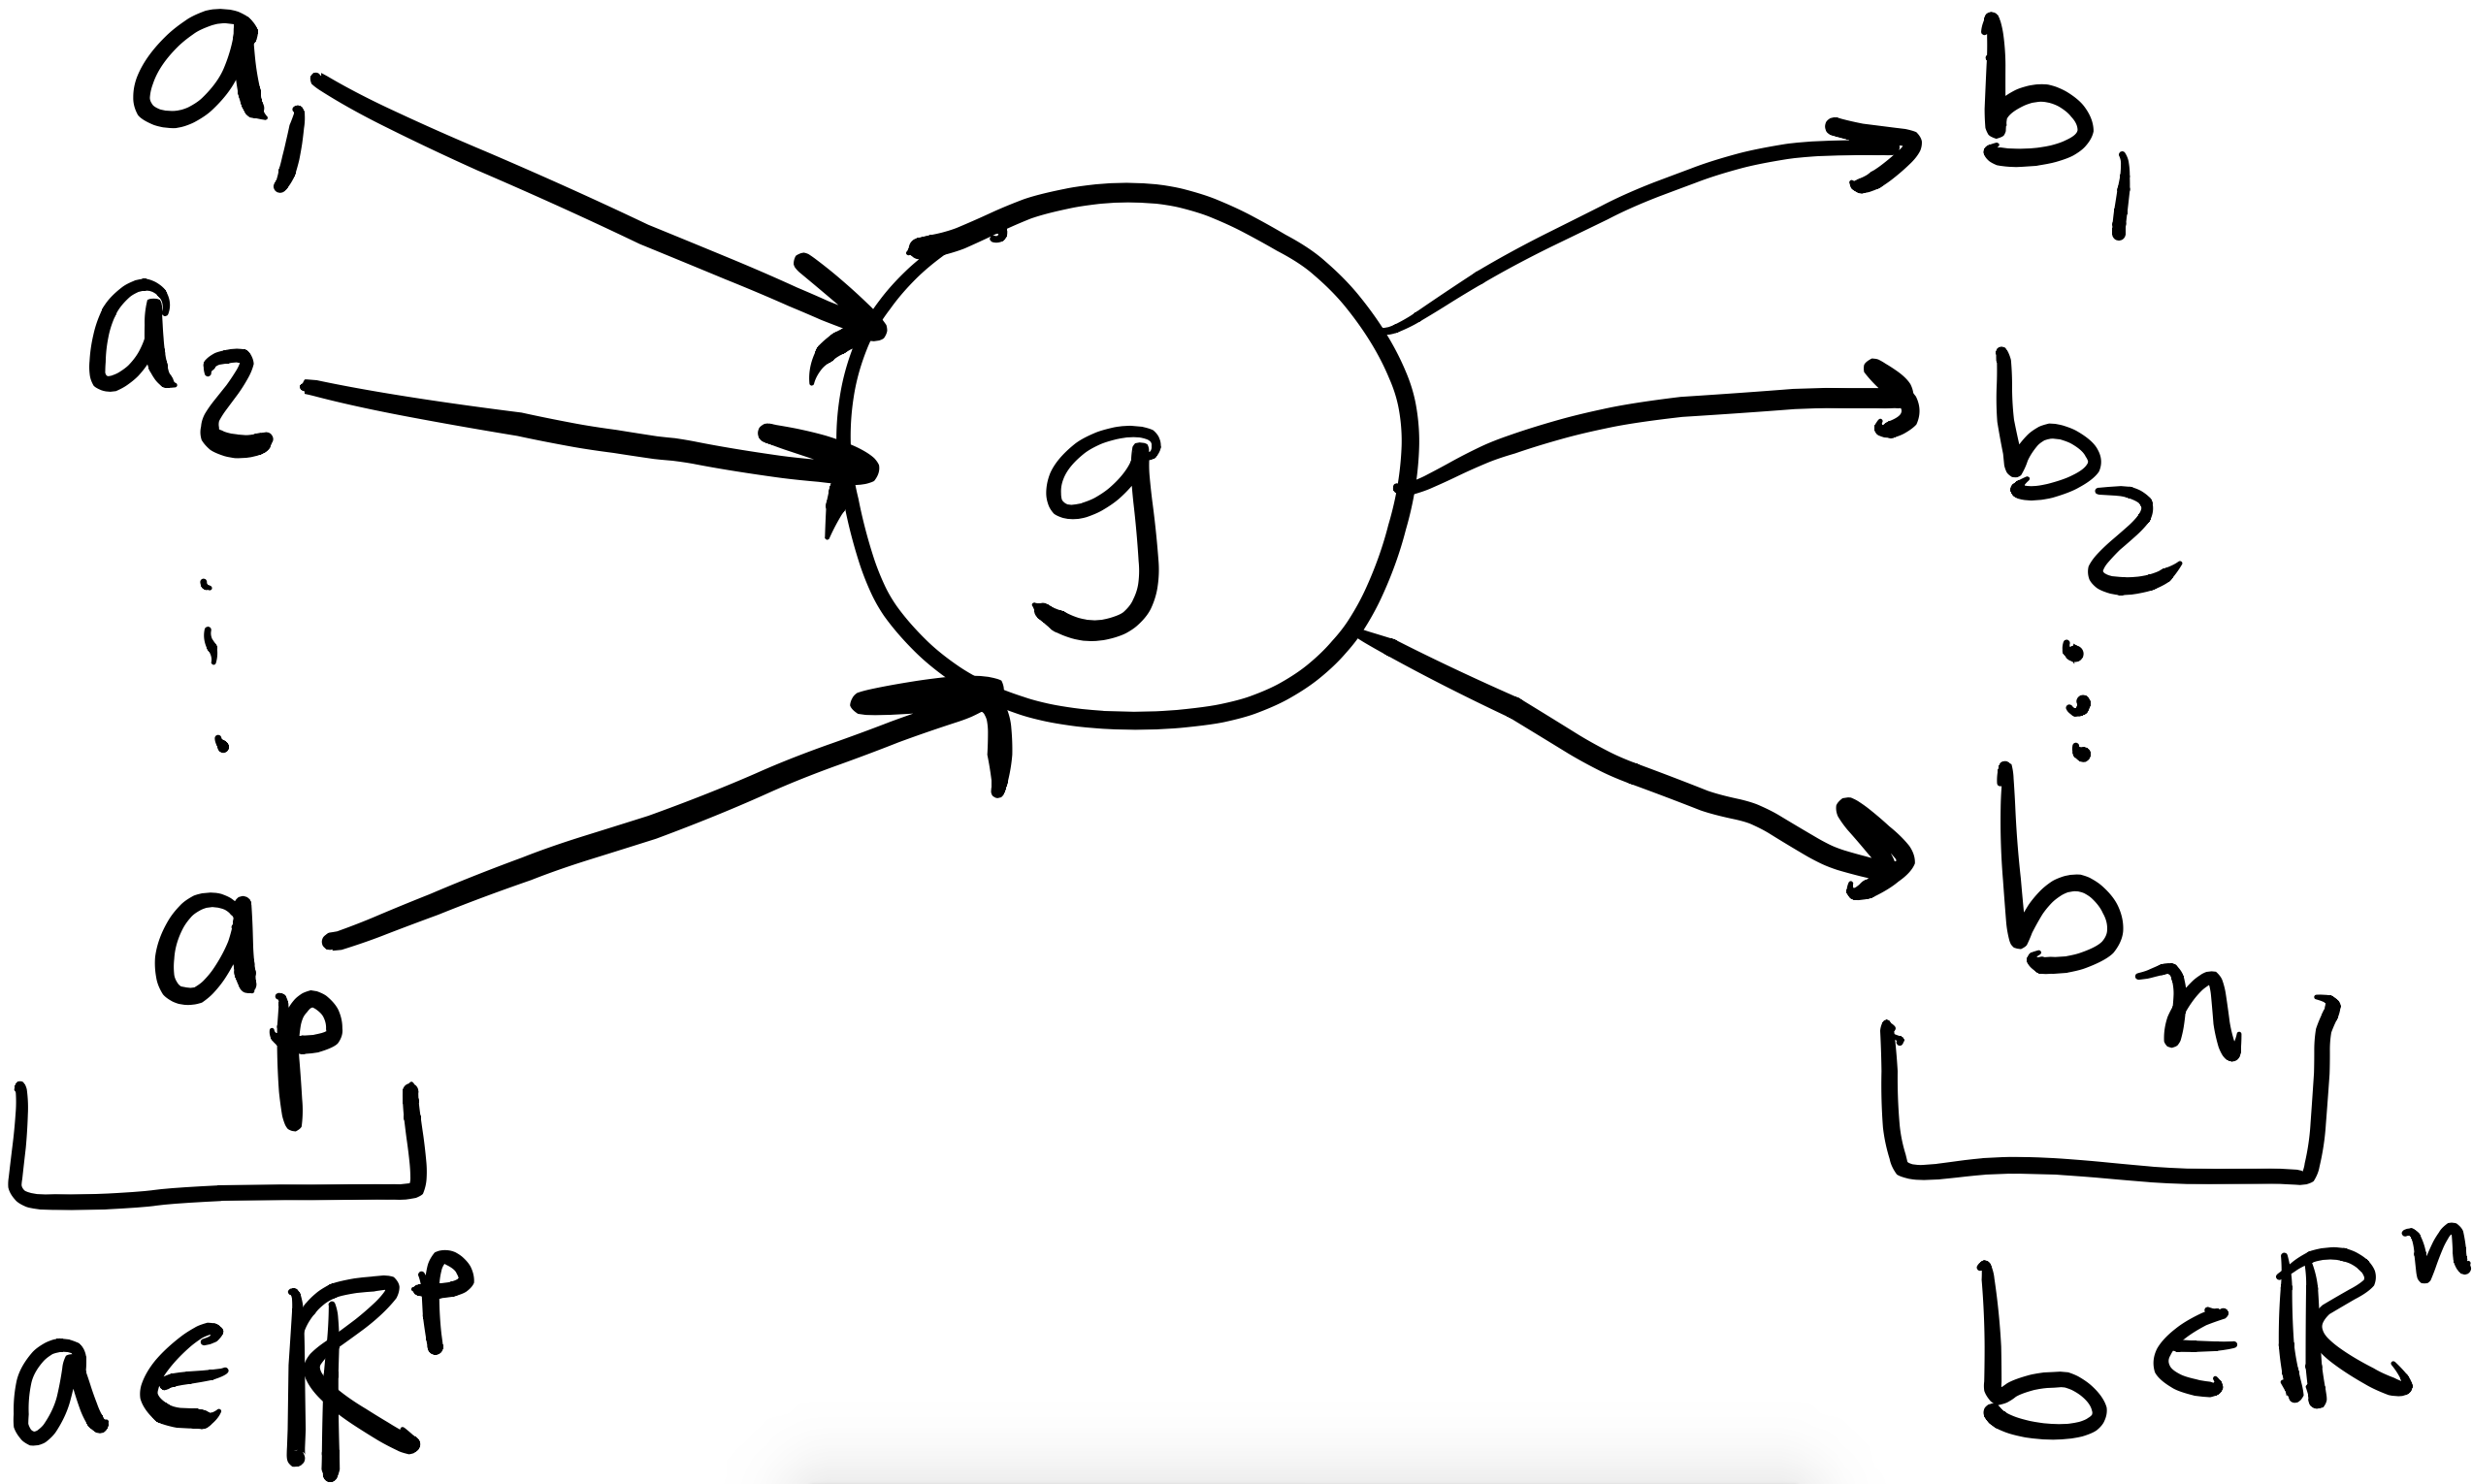
\includegraphics[scale=0.0625]{figures/one-fn-comp-graph-partials}
\end{figure}

\onslide<+->{
\column{.5\textwidth}
\begin{itemize}[<+->]
\item Let $b=g(a)=Ma+c$. What is $b_{i}$?
\item $b_{i}$ depends on the $i$th row of $M$: 
\[
b_{i}=\sum_{k=1}^{p}M_{ik}a_{k}+c_{i} .
\]
\item If $a_j \leftarrow a_j + {\color{blue}\delta}$, what is $b_i$?
\[
b_i \leftarrow b_i + {\color{blue}M_{ij}\delta} .
\]
\end{itemize}
}
\end{columns}
\onslide<+->{
Partial derivative/gradient measures \emph{sensitivity}:
If we perturb an input a little bit, how much does an output change?
}
\note[item]{Now, what is the meaning of partial derivatives on this graph. Let's consider the affine function as an example.}
\note[item]{Write the function.}
\note[item]{Draw matrix multiplication.}
\note[item]{$M_{ij} = \frac{\partial b_i}{\partial a_j}$}
\end{frame}

\begin{frame}{Partial Derivatives in general}
\begin{itemize}
\item Consider a function $g:\reals^{p}\to\reals^{n}$.
\end{itemize}
\begin{columns}[t]

\column{.35\textwidth}
\begin{figure}
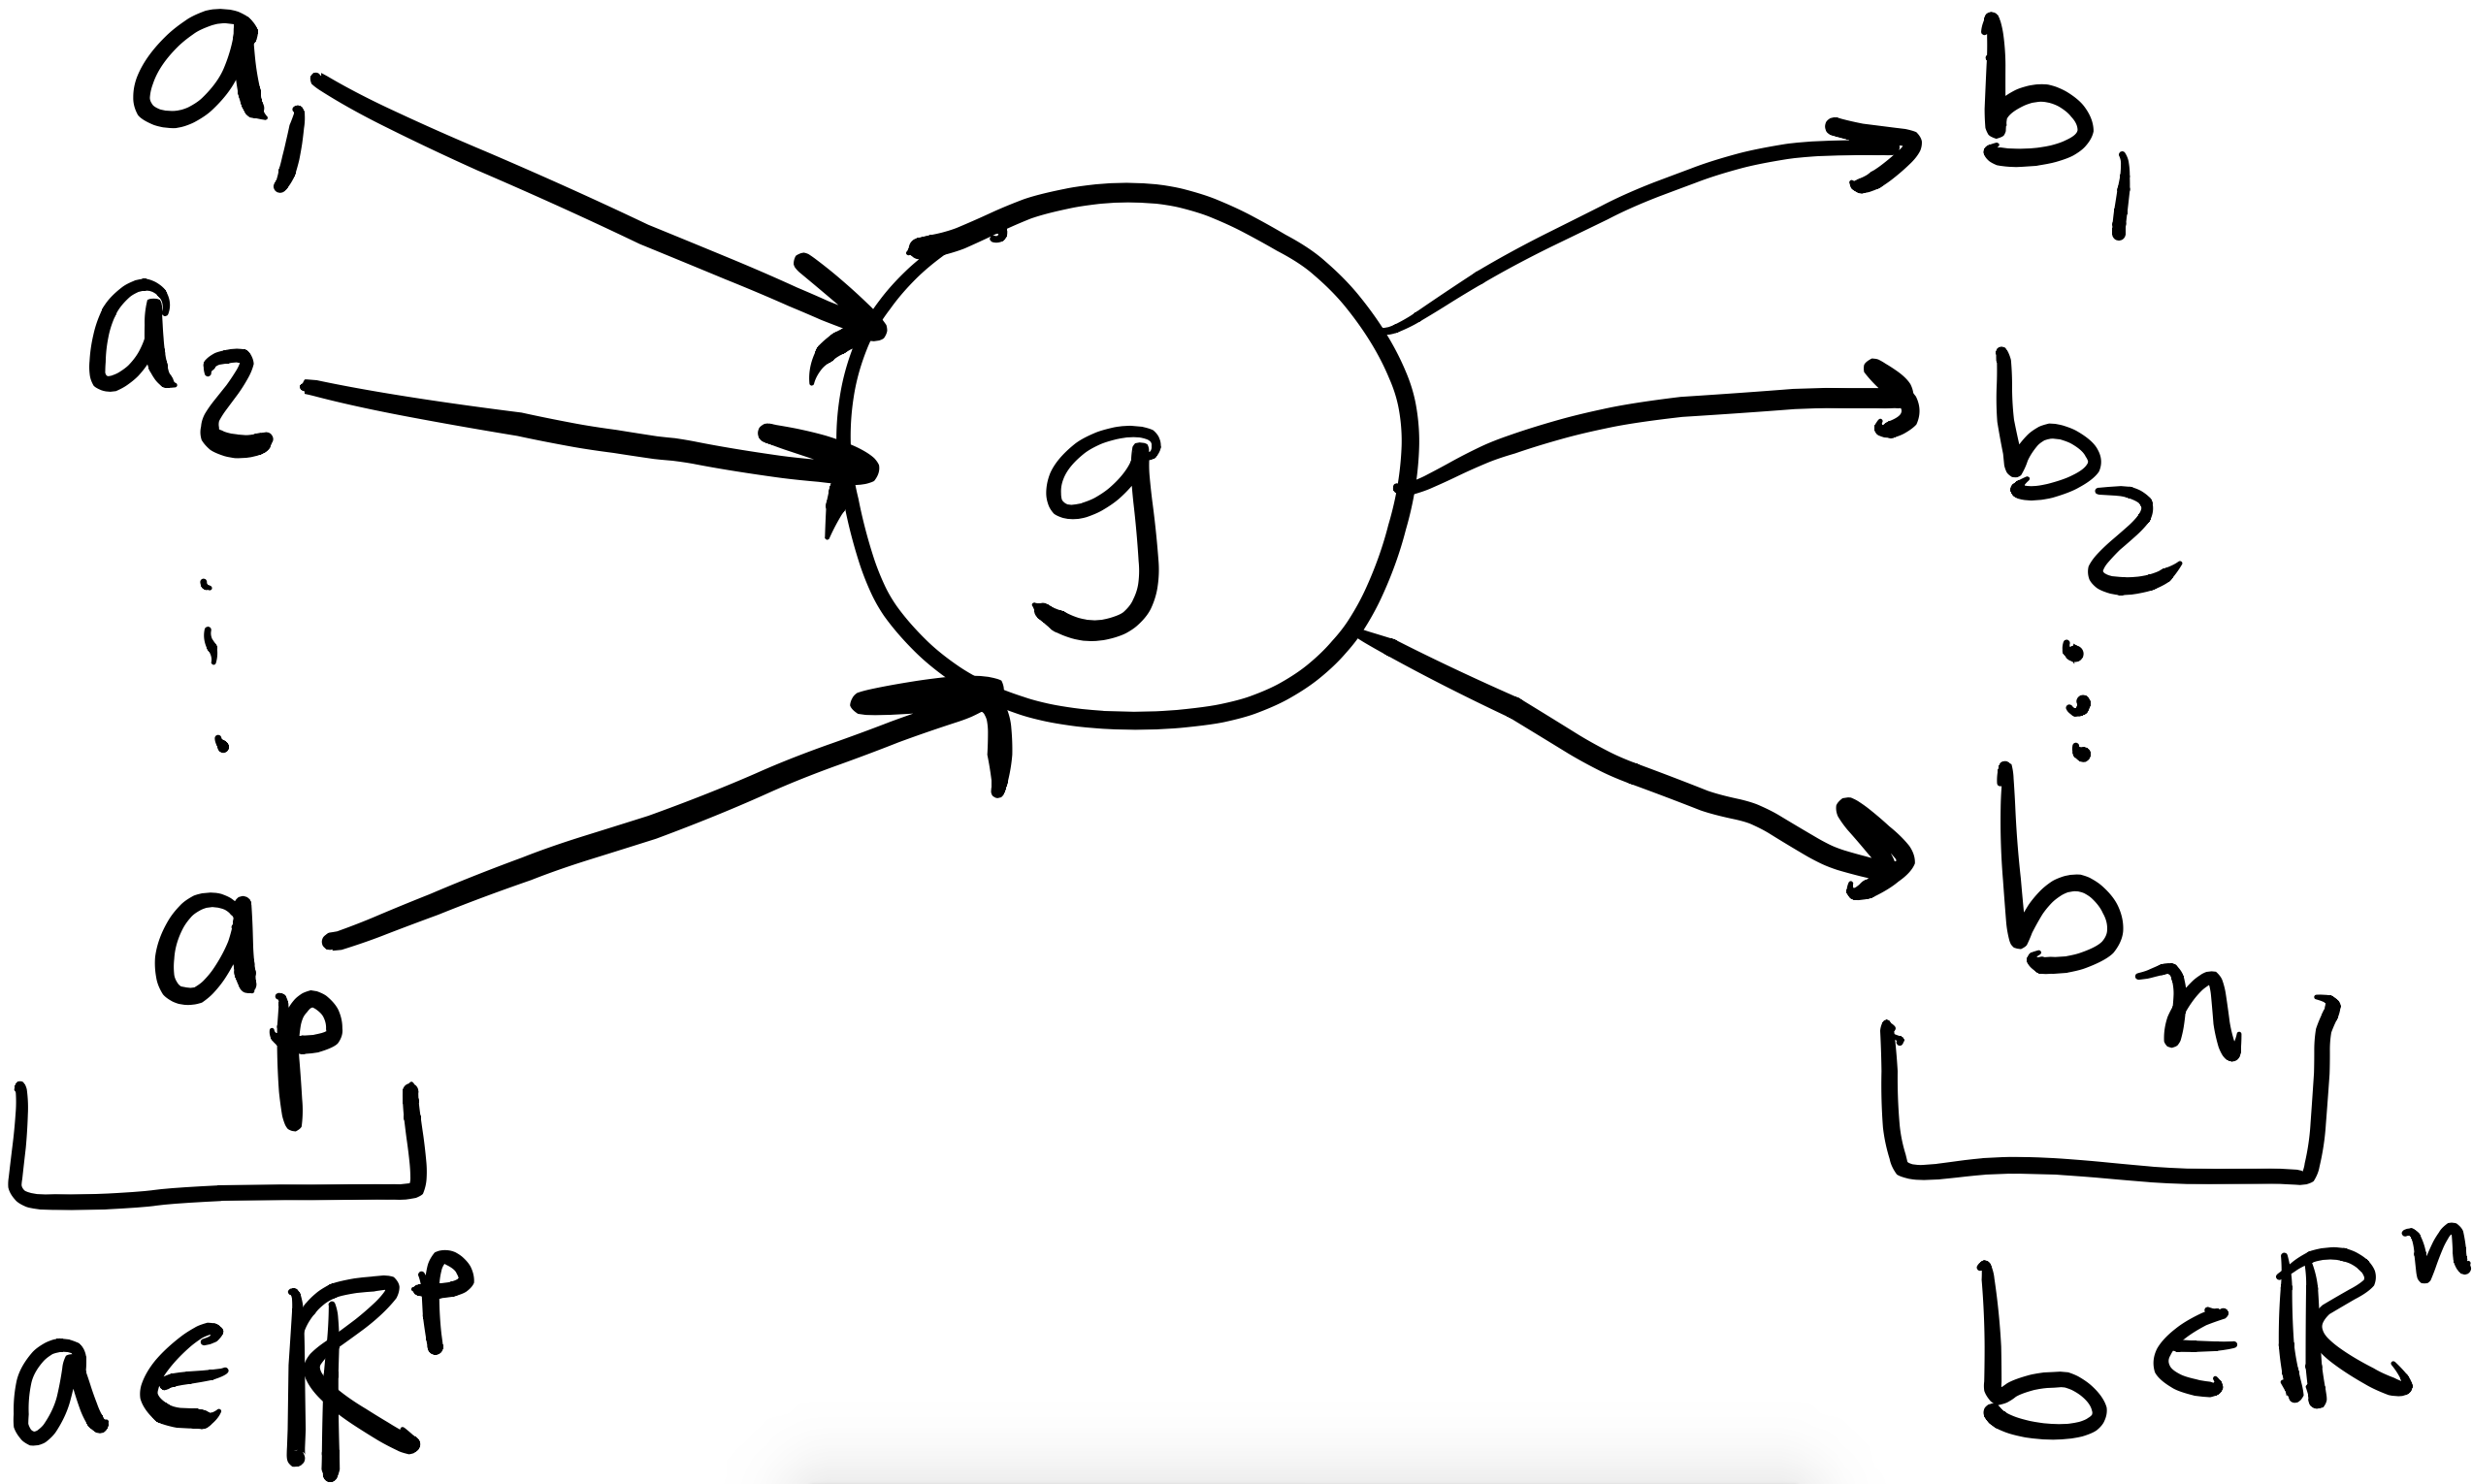
\includegraphics[scale=0.07]{figures/one-fn-comp-graph-partials}
\end{figure}

\column{.5\textwidth}
\begin{itemize}
\item Partial derivative $\frac{\partial b_{i}}{\partial a_{j}}$ is the
instantaneous rate of change of $b_{i}$ as we change $a_{j}$.
\item If we change $a_{j}$ slightly to
\[
a_{j}+{\color{blue}\delta} ,
\]
\item Then (for small $\delta$), $b_{i}$ changes to approximately
\[
b_{i}+{\color{blue}\frac{\partial b_{i}}{\partial a_{j}}\delta} .
\]
\end{itemize}
\end{columns}

\end{frame}

\begin{frame}
{Compose multiple functions}
\begin{itemize}
\item Compose two functions $g:\reals^{p}\to\reals^{n}$ and $f:\reals^{n}\to\reals^{m}$.
\item $b=g(a)$, $c=f(b)$.
\end{itemize}
\begin{columns}
\begin{column}{0.5\textwidth}
\begin{figure}
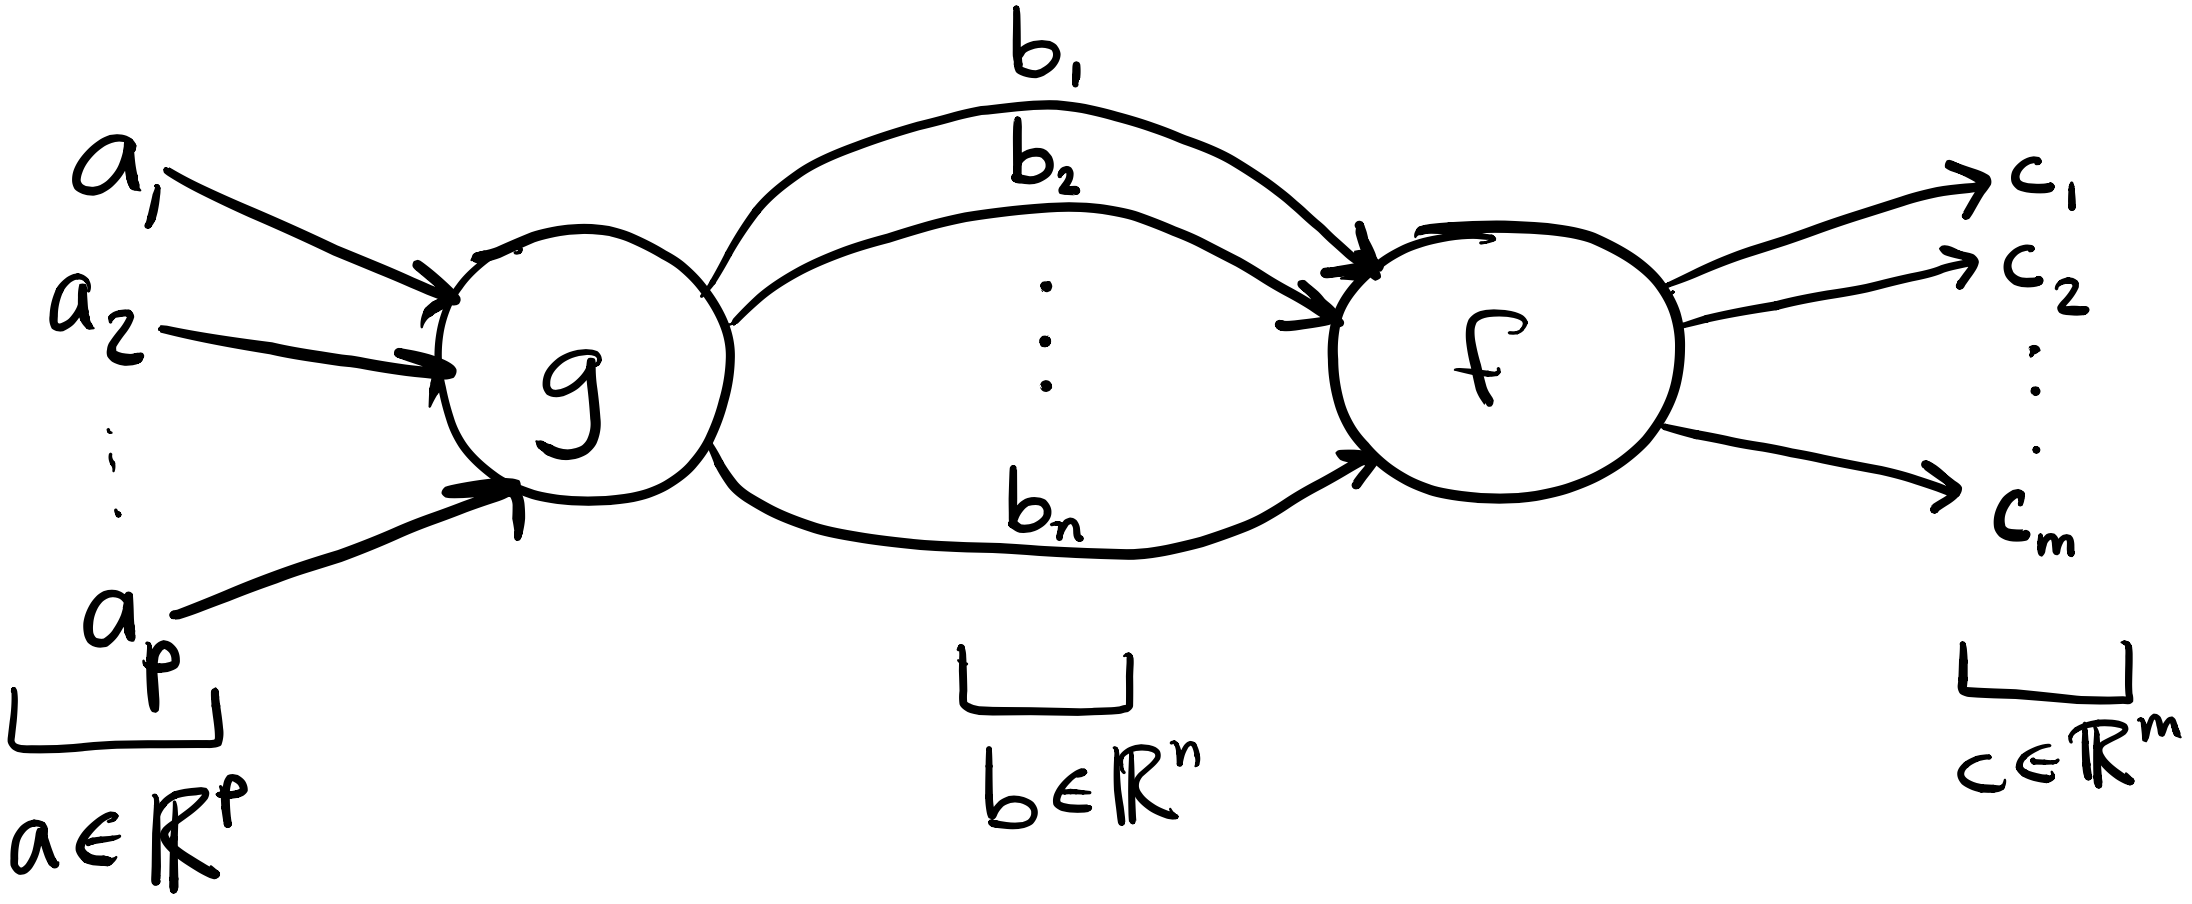
\includegraphics[width=1\columnwidth]{figures/two-fn-comp-graph-partials}
\end{figure}
\end{column}

\begin{column}{0.5\textwidth}
\begin{itemize}[<+->]
\item How does change in $a_j$ affect $c_i$?
\item Visualize \textbf{chain rule}:
\begin{itemize}[<.->]
\item \textcolor{blue}{Sum} changes induced on all paths from $a_j$ to $c_i$.
\item Changes on one path is the {\color{red}product} of changes on each edge along the path.
\onslide<+->{
\[
\frac{\partial c_{i}}{\partial a_{j}}={\color{blue}\sum_{k=1}^{n}}
{\color{red} \frac{\partial c_{i}}{\partial b_{k}}\frac{\partial b_{k}}{\partial a_{j}}} .
\]
}
\end{itemize} 
\end{itemize}
\end{column}
\end{columns}
\note[item]{In math, we know that $c=f(g(z))$, so that we can use chain rule. But how do we visualize chain rule on this graph?}
\note[item]{$a_j$ would affect $b_1$ to $b_n$, and each $b_k$ further affects $c_i$}.
\end{frame}

\subsection{Example Computation Graphs}
\begin{frame}{Example: Linear least squares}
\begin{itemize}
\item Hypothesis space $\left\{ f(x)=w^{T}x+b\mid w\in\reals^{d},b\in\reals\right\} $.

\item Data set $\left(x_{1},y_{1}\right),\ldots,\left(x_{n},y_{n}\right)\in\reals^{d}\times\reals$.
\item Define
\[
\ell_{i}(w,b)=\left[\left(w^{T}x_{i}+b\right)-y_{i}\right]^{2}.
\]


\pause{}
\item In SGD, in each round we'd choose a random index $i\in1,\ldots,n$
and take a gradient step
\begin{eqnarray*}
w_{j} & \gets & w_{j}-\eta\frac{\partial\ell_{i}(w,b)}{\partial w_{j}}\text{, for }j=1,\ldots,d\\
b & \gets & b-\eta\frac{\partial\ell_{i}(w,b)}{\partial b},
\end{eqnarray*}
for some step size $\eta>0$.
\item Let's see how to calculate these partial derivatives on a computation graph.
\end{itemize}
\end{frame}
%
\begin{frame}{Computation Graph and Intermediate Variables}
\begin{itemize}
\item For a generic training point $\left(x,y\right)$, denote the loss
by 
\[
\ell(w,b)=\left[\left(w^{T}x+b\right)-y\right]^{2}.
\]
\pause
\item Let's break this down into some intermediate computations:
\begin{columns}[t]

\column{.35\textwidth}

\begin{eqnarray*}
\text{(prediction) }\hat{y} & = & \sum_{j=1}^{d}w_{j}x_{j}+b\\
\pause\text{(residual) }r & = & y-\hat{y}\\
\pause\text{(loss) }\ell & = & r^{2}
\end{eqnarray*}


\pause{}

\column{.65\textwidth}
\begin{center}
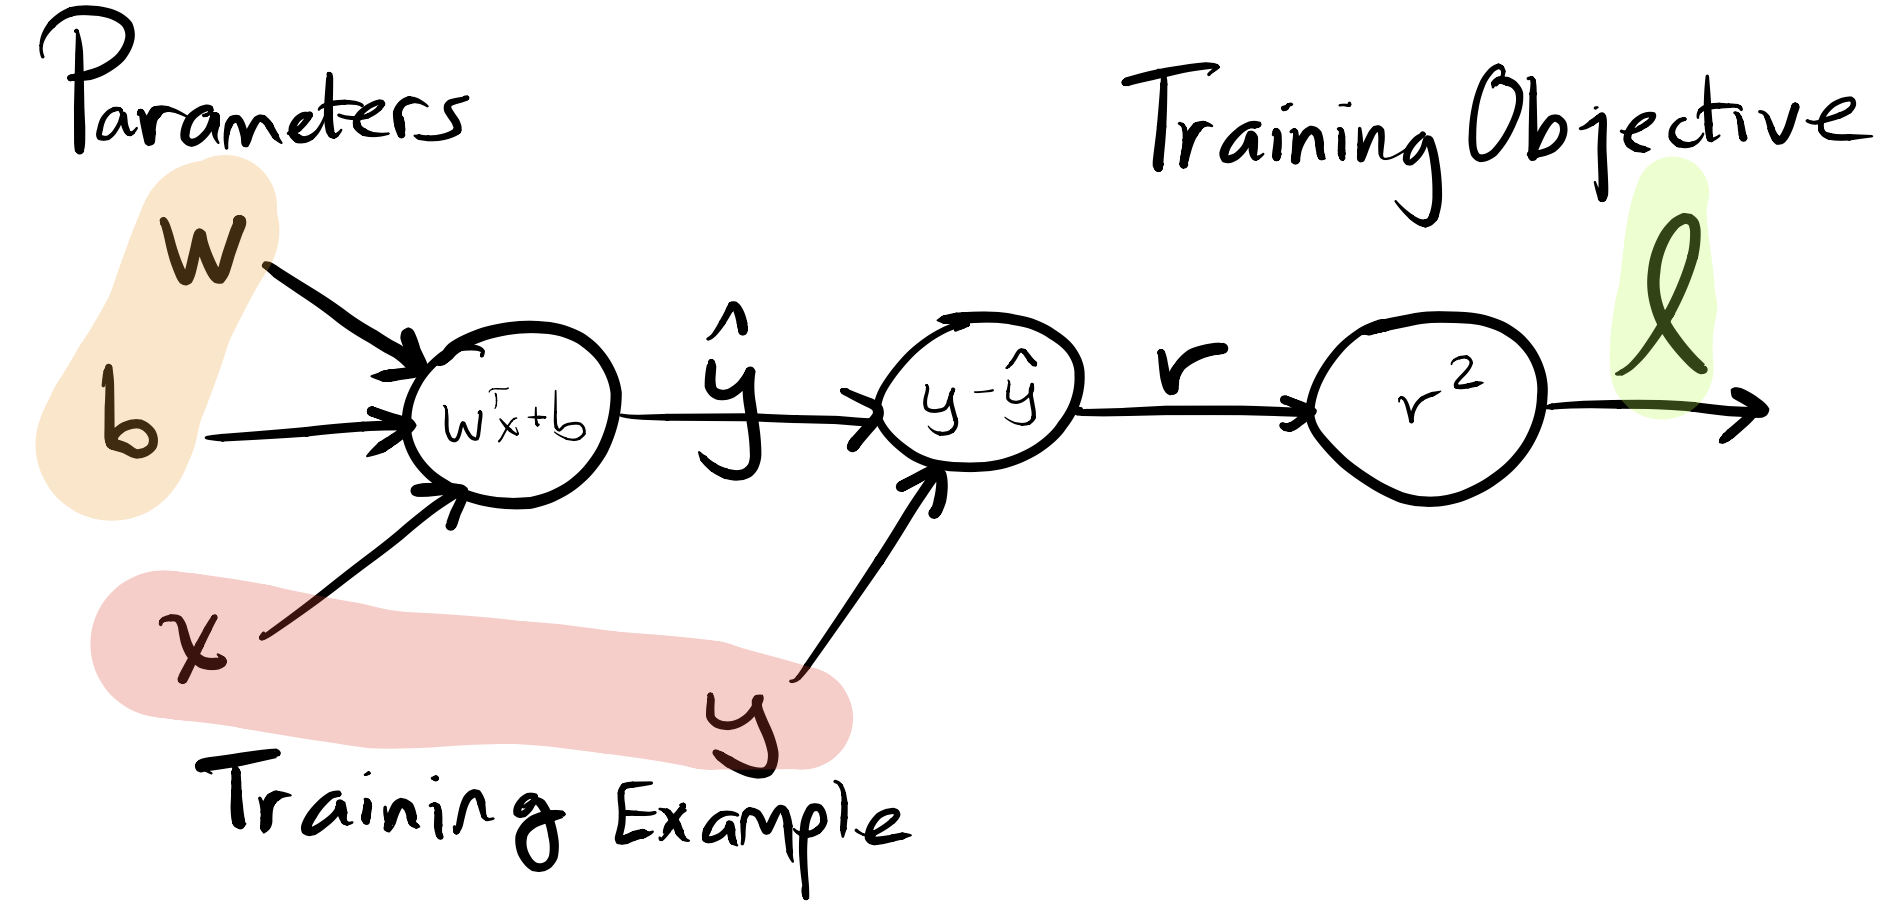
\includegraphics[height=0.45\textheight]{figures/linear-sqr-loss-comp-graph-labels}
\par\end{center}

\end{columns}

\end{itemize}
\end{frame}
%
\begin{frame}{Partial Derivatives on Computation Graph}
\begin{itemize}
\item We'll work our way from graph output $\ell$ back to the parameters
$w$ and $b$:
\begin{columns}[c]

\column{.45\textwidth}

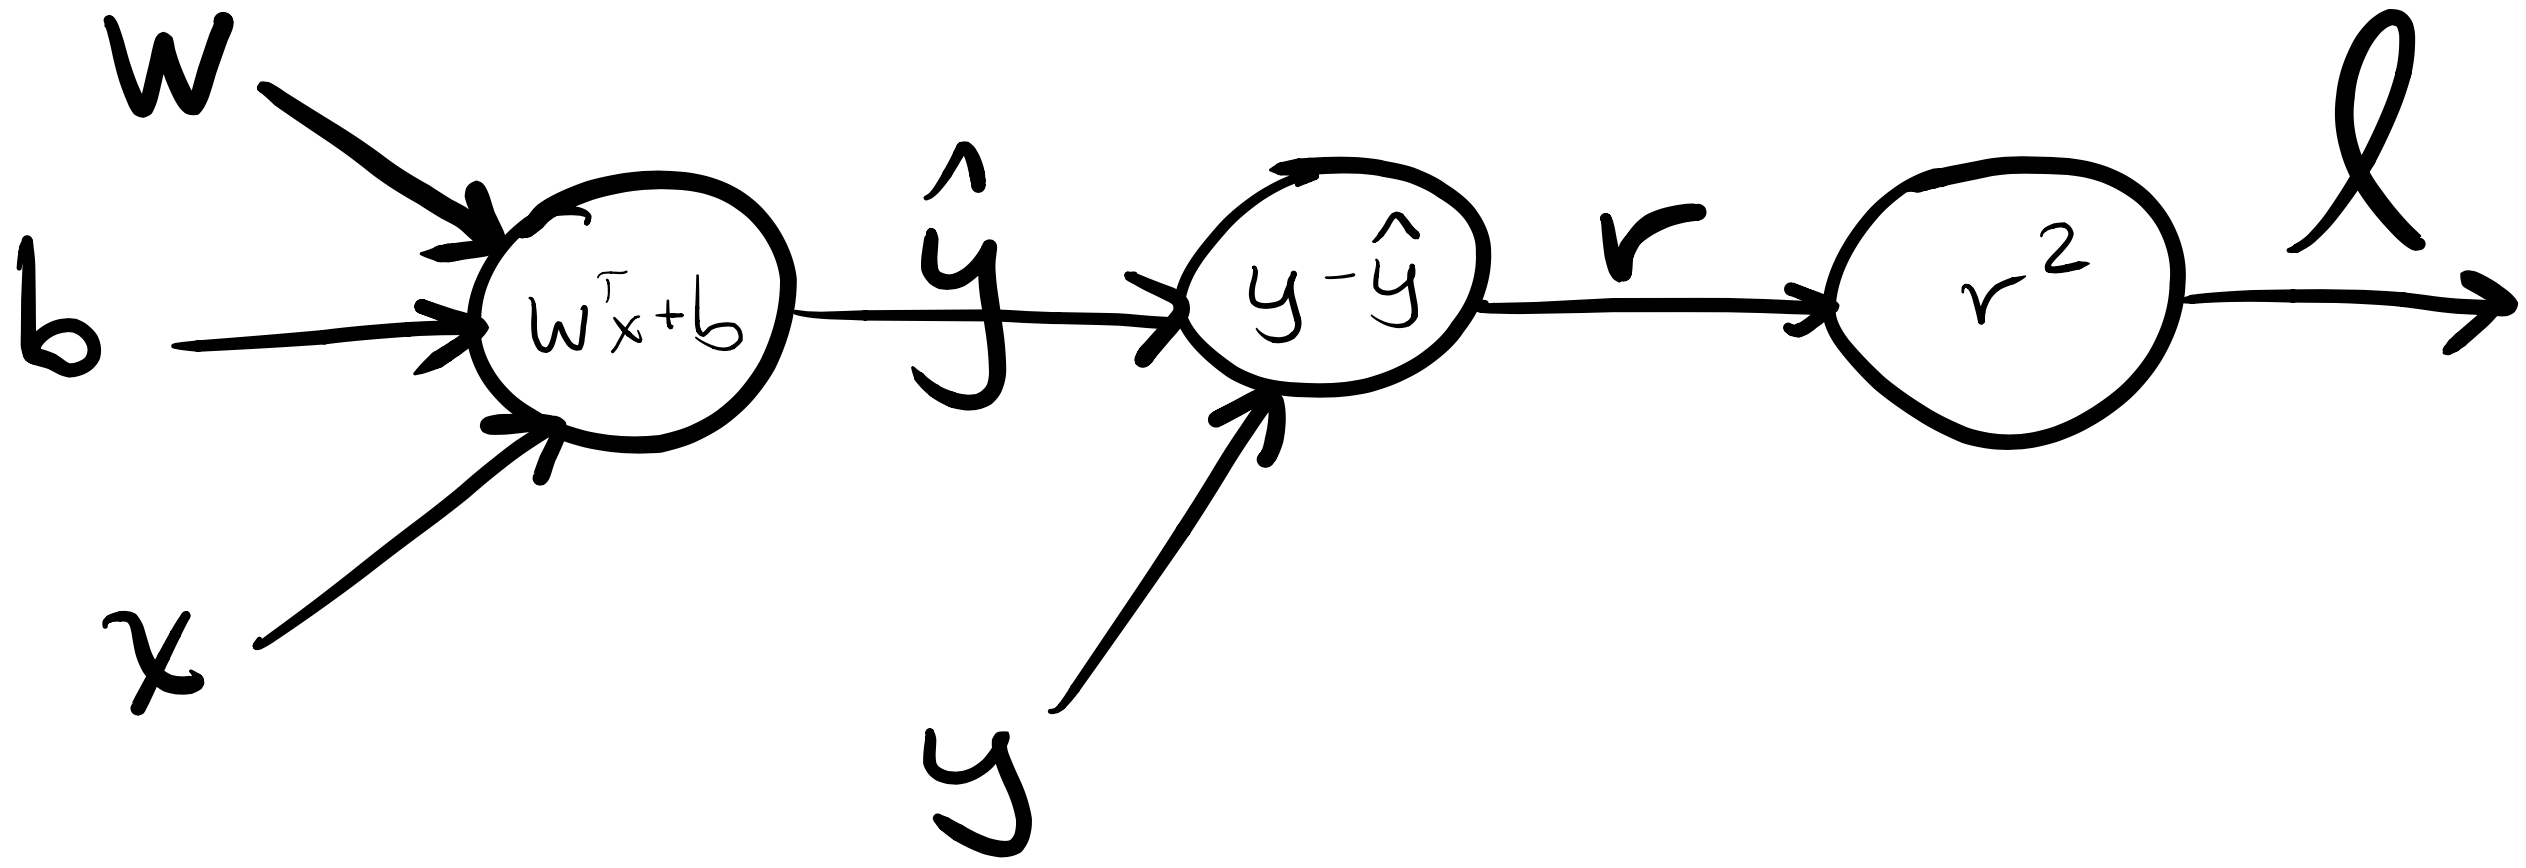
\includegraphics[width=1\columnwidth]{figures/linear-sqr-loss-comp-graph}

\pause{}

\column{.45\textwidth}

\begin{eqnarray*}
\frac{\partial\ell}{\partial r} & = & \pause2r\\
\frac{\partial\ell}{\partial\hat{y}} & = & \pause\frac{\partial\ell}{\partial r}\frac{\partial r}{\partial\hat{y}}=\left(2r\right)(-1)=-2r\\
\frac{\partial\ell}{\partial b} & = & \pause\frac{\partial\ell}{\partial\hat{y}}\frac{\partial\hat{y}}{\partial b}=\left(-2r\right)(1)=-2r\\
\frac{\partial\ell}{\partial w_{j}} & = & \pause\frac{\partial\ell}{\partial\hat{y}}\frac{\partial\hat{y}}{\partial w_{j}}=\left(-2r\right)x_{j}=-2rx_{j}
\end{eqnarray*}

\end{columns}

\end{itemize}
\note[item]{Notice that in each step we can use previous results.}
\end{frame}

\begin{frame}{Example: Ridge Regression}
\begin{itemize}
\item For training point $\left(x,y\right)$, the $\ell_{2}$-regularized
objective function is 
\[
J(w,b)=\left[\left(w^{T}x+b\right)-y\right]^{2}+\lambda w^{T}w.
\]
\item Let's break this down into some intermediate computations:
\begin{columns}[t]

\column{.35\textwidth}

\begin{eqnarray*}
\text{(prediction) }\hat{y} & = & \sum_{j=1}^{d}w_{j}x_{j}+b\\
\text{(residual) }r & = & y-\hat{y}\\
\text{(loss) }\ell & = & r^{2}\\
\pause\text{(regularization) }R & = & \lambda w^{T}w\\
\text{(objective) }J & = & \ell+R
\end{eqnarray*}


\pause{}

\column{.65\textwidth}
\begin{center}
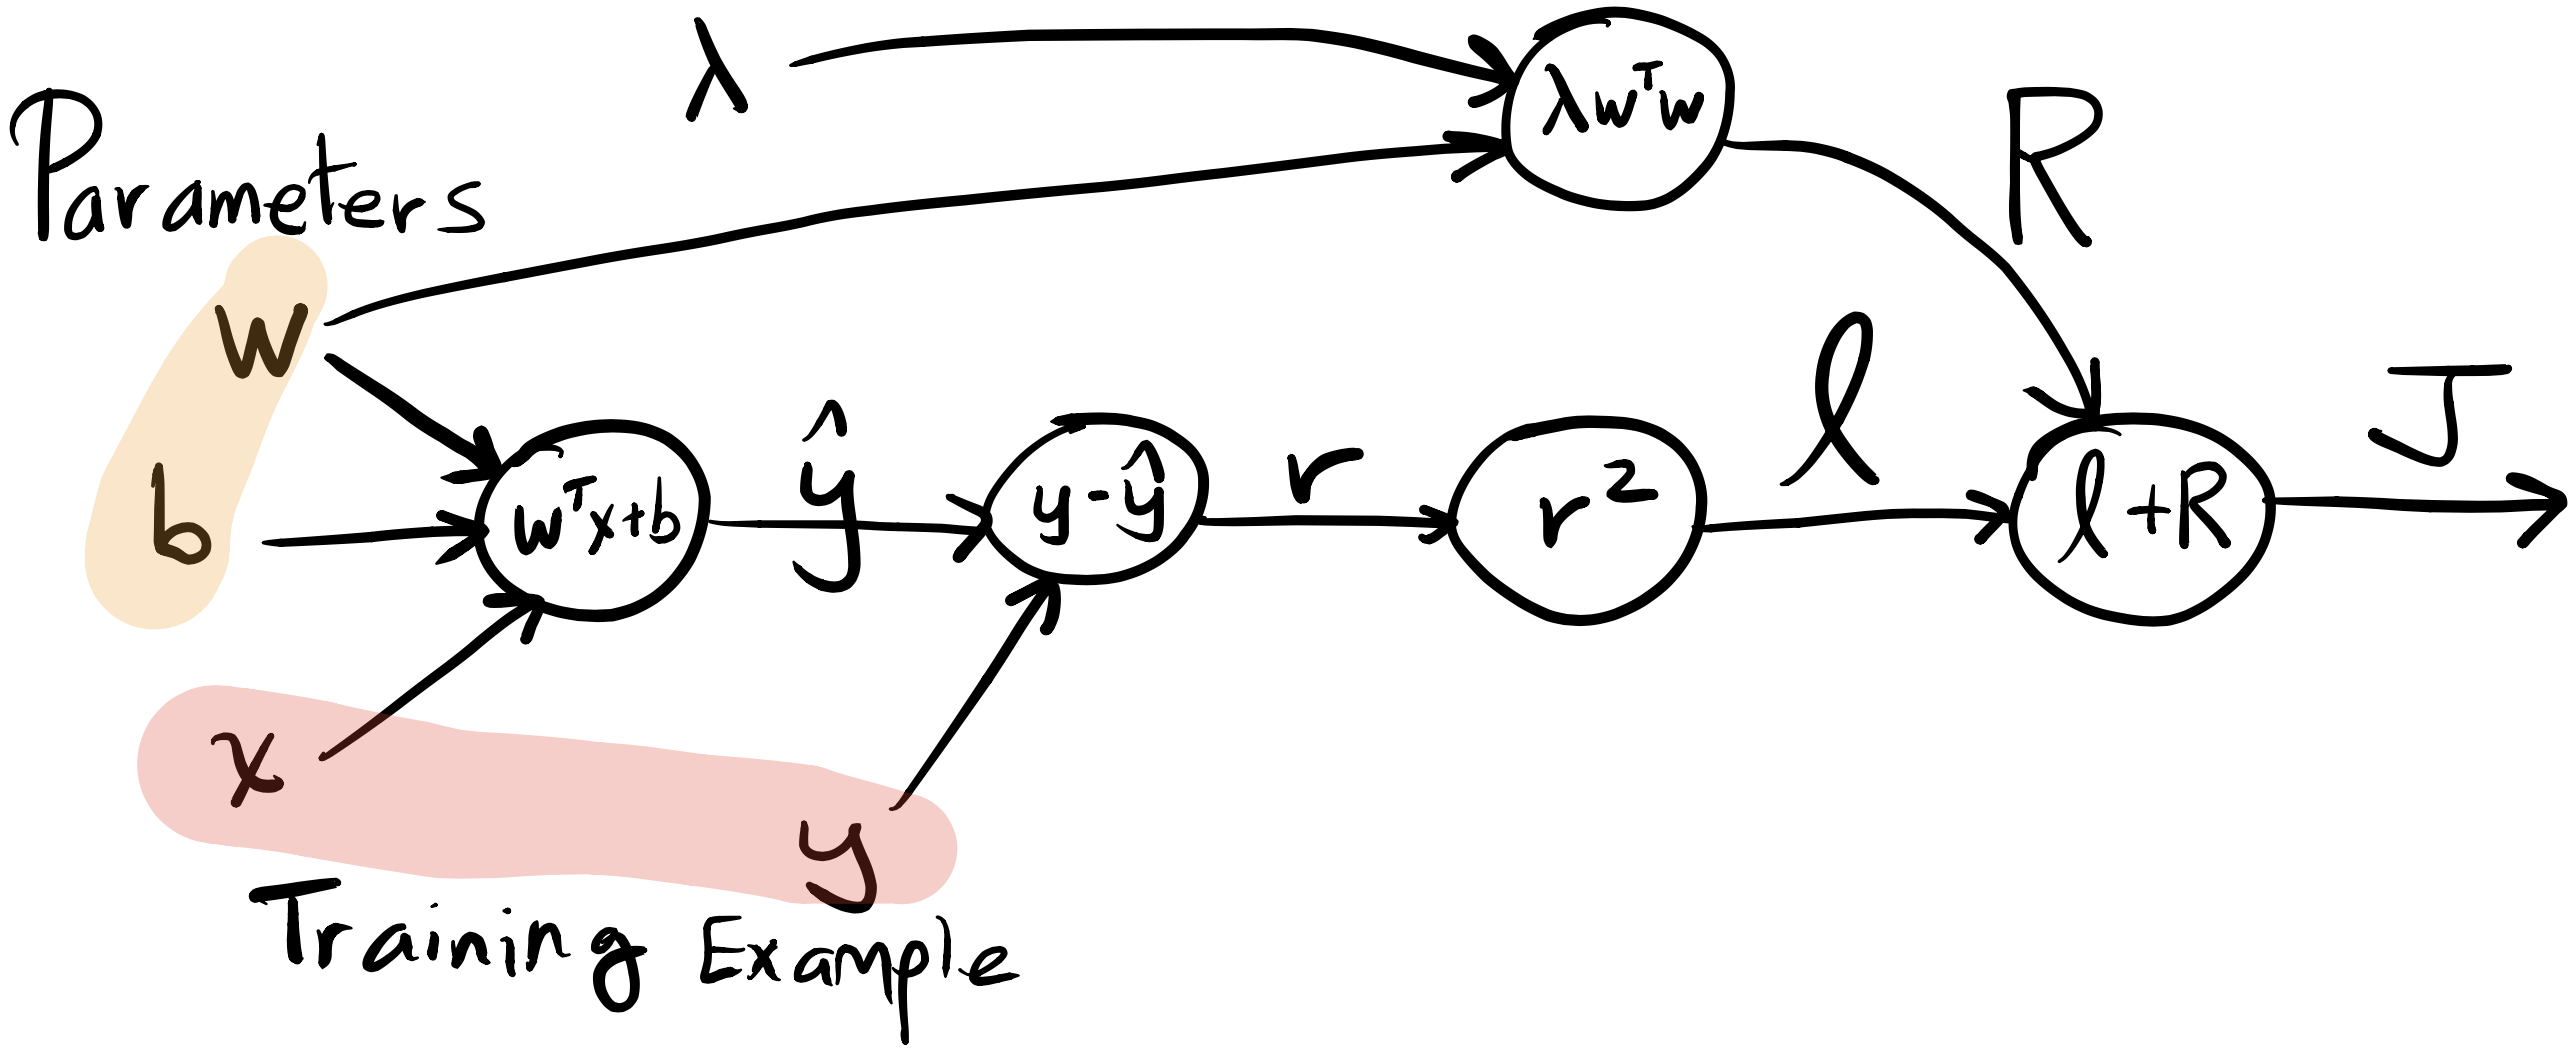
\includegraphics[height=0.45\textheight]{figures/ridge-regression-comp-graph-labels}
\par\end{center}

\end{columns}

\end{itemize}
\end{frame}
%
\begin{frame}{Partial Derivatives on Computation Graph}
\begin{itemize}
\item We'll work our way from graph output $\ell$ back to the parameters
$w$ and $b$:
\begin{columns}[c]

\column{.55\textwidth}

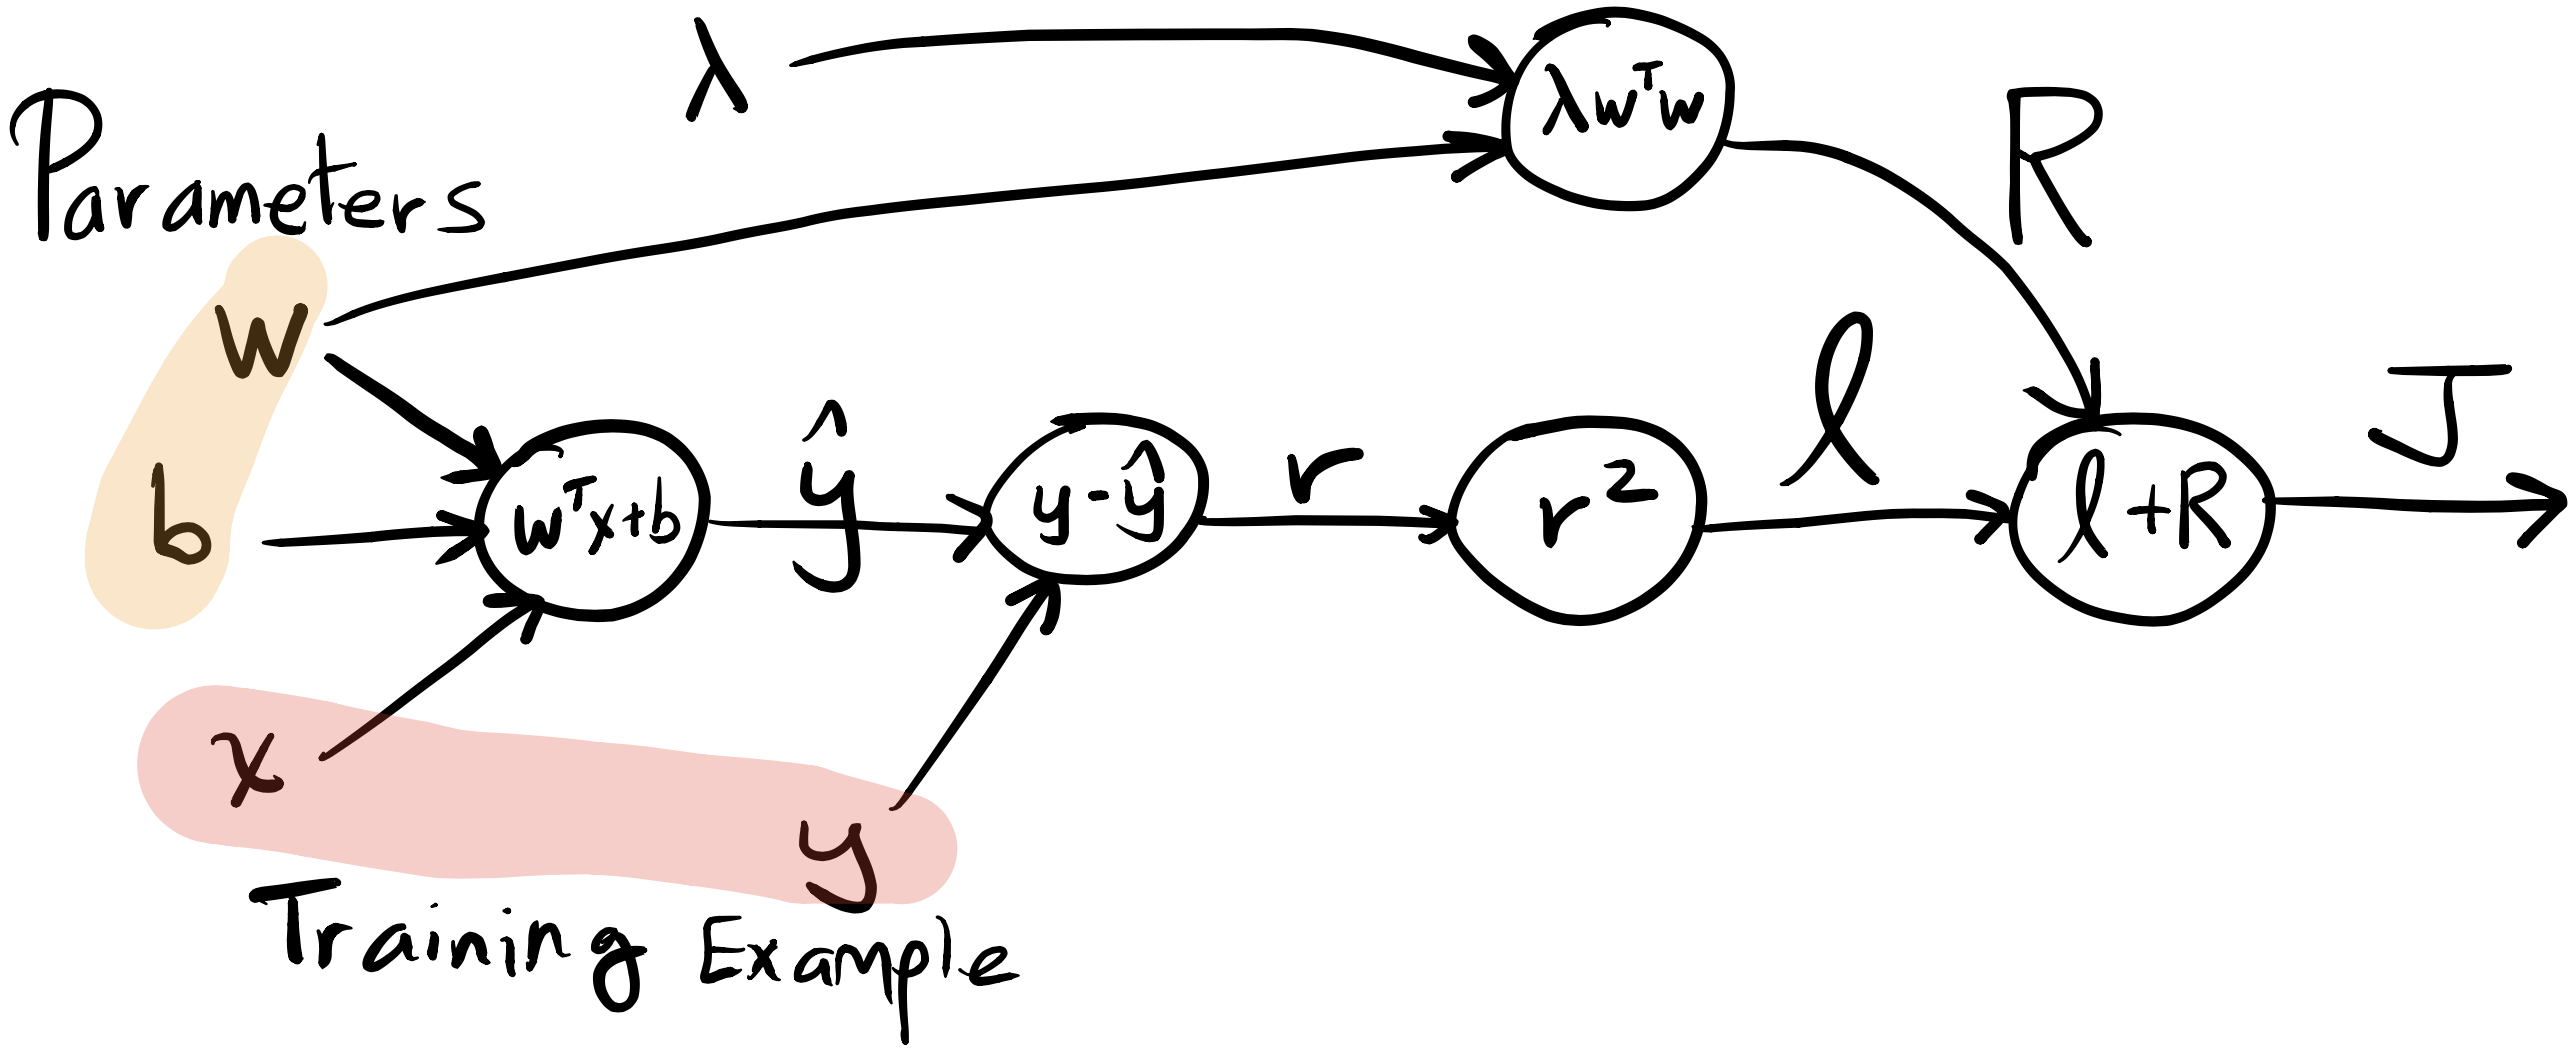
\includegraphics[width=1\columnwidth]{figures/ridge-regression-comp-graph-labels}


\column{.45\textwidth}

\begin{eqnarray*}
\frac{\partial J}{\partial\ell} & = & \frac{\partial J}{\partial R}=1\\
\frac{\partial J}{\partial\hat{y}} & = & \frac{\partial J}{\partial\ell}\frac{\partial\ell}{\partial r}\frac{\partial r}{\partial\hat{y}}=\left(1\right)(2r)\left(-1\right)=-2r\\
\frac{\partial J}{\partial b} & = & \frac{\partial J}{\partial\hat{y}}\frac{\partial\hat{y}}{\partial b}=\left(-2r\right)\left(1\right)=-2r\\
\frac{\partial J}{\partial w_{j}} & = & \text{\think{Exercise}} 
\end{eqnarray*}

\end{columns}

\end{itemize}
\end{frame}
%
%\begin{frame}{Handling Nodes with Multiple Children}
%\begin{itemize}
%\item Consider $a\mapsto J=h(f(a),g(a))$.
%\end{itemize}
%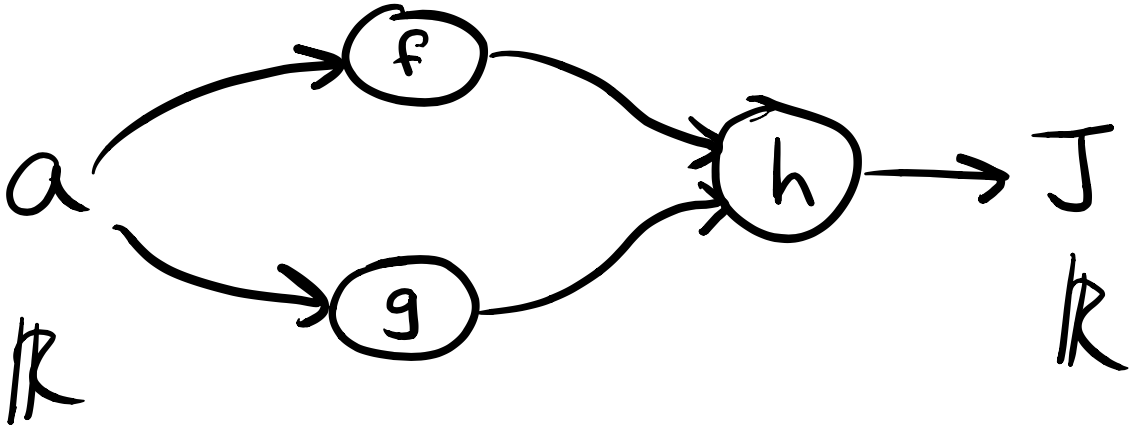
\includegraphics[height=0.3\textheight]{figures/split-output}
%\begin{itemize}
%\item It's helpful to think about having two independent copies of $a$,
%call them $a^{(1)}$ and $a^{(2)}$...
%\end{itemize}
%\end{frame}
%%
%\begin{frame}{Handling Nodes with Multiple Children}
%\begin{columns}[c]
%
%\column{.45\textwidth}
%
%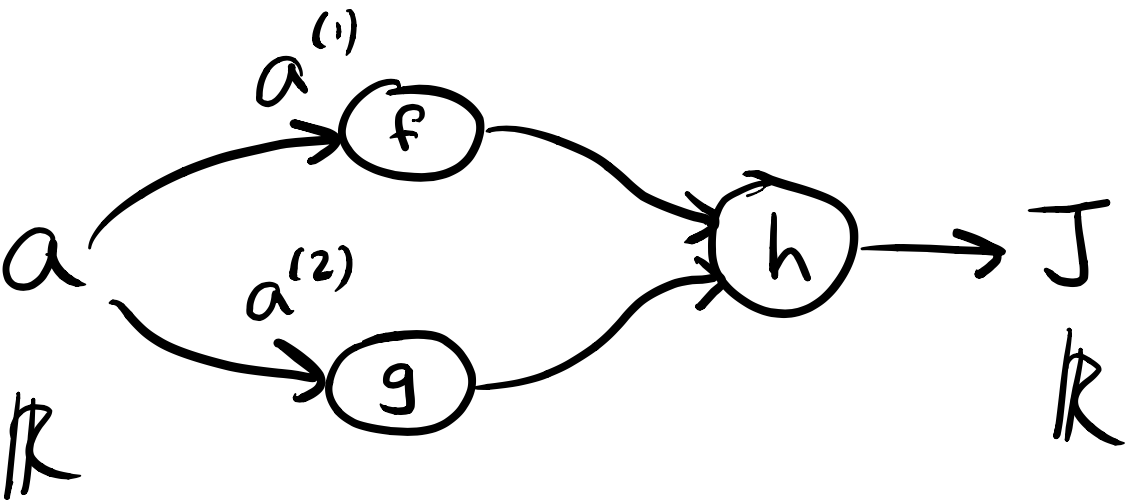
\includegraphics[width=1\columnwidth]{figures/split-output-2copies}
%
%\pause{}
%
%\column{.45\textwidth}
%
%\begin{eqnarray*}
%\frac{\partial J}{\partial a} & = & \pause\frac{\partial J}{\partial a^{(1)}}\frac{\partial a^{(1)}}{\partial a}+\frac{\partial J}{\partial a^{(2)}}\frac{\partial a^{(2)}}{\partial a}\\
% & = & \pause\frac{\partial J}{\partial a^{(1)}}+\frac{\partial J}{\partial a^{(2)}}
%\end{eqnarray*}
%
%\end{columns}
%
%\begin{itemize}
%\item Derivative w.r.t. $a$ is the sum of derivatives w.r.t. each copy
%of $a$.
%\end{itemize}
%\end{frame}
%%
%\begin{frame}{Partial Derivatives on Computation Graph}
%\begin{itemize}
%\item We'll work our way from graph output $\ell$ back to the parameters
%$w$ and $b$:
%\begin{columns}[c]
%
%\column{.45\textwidth}
%
%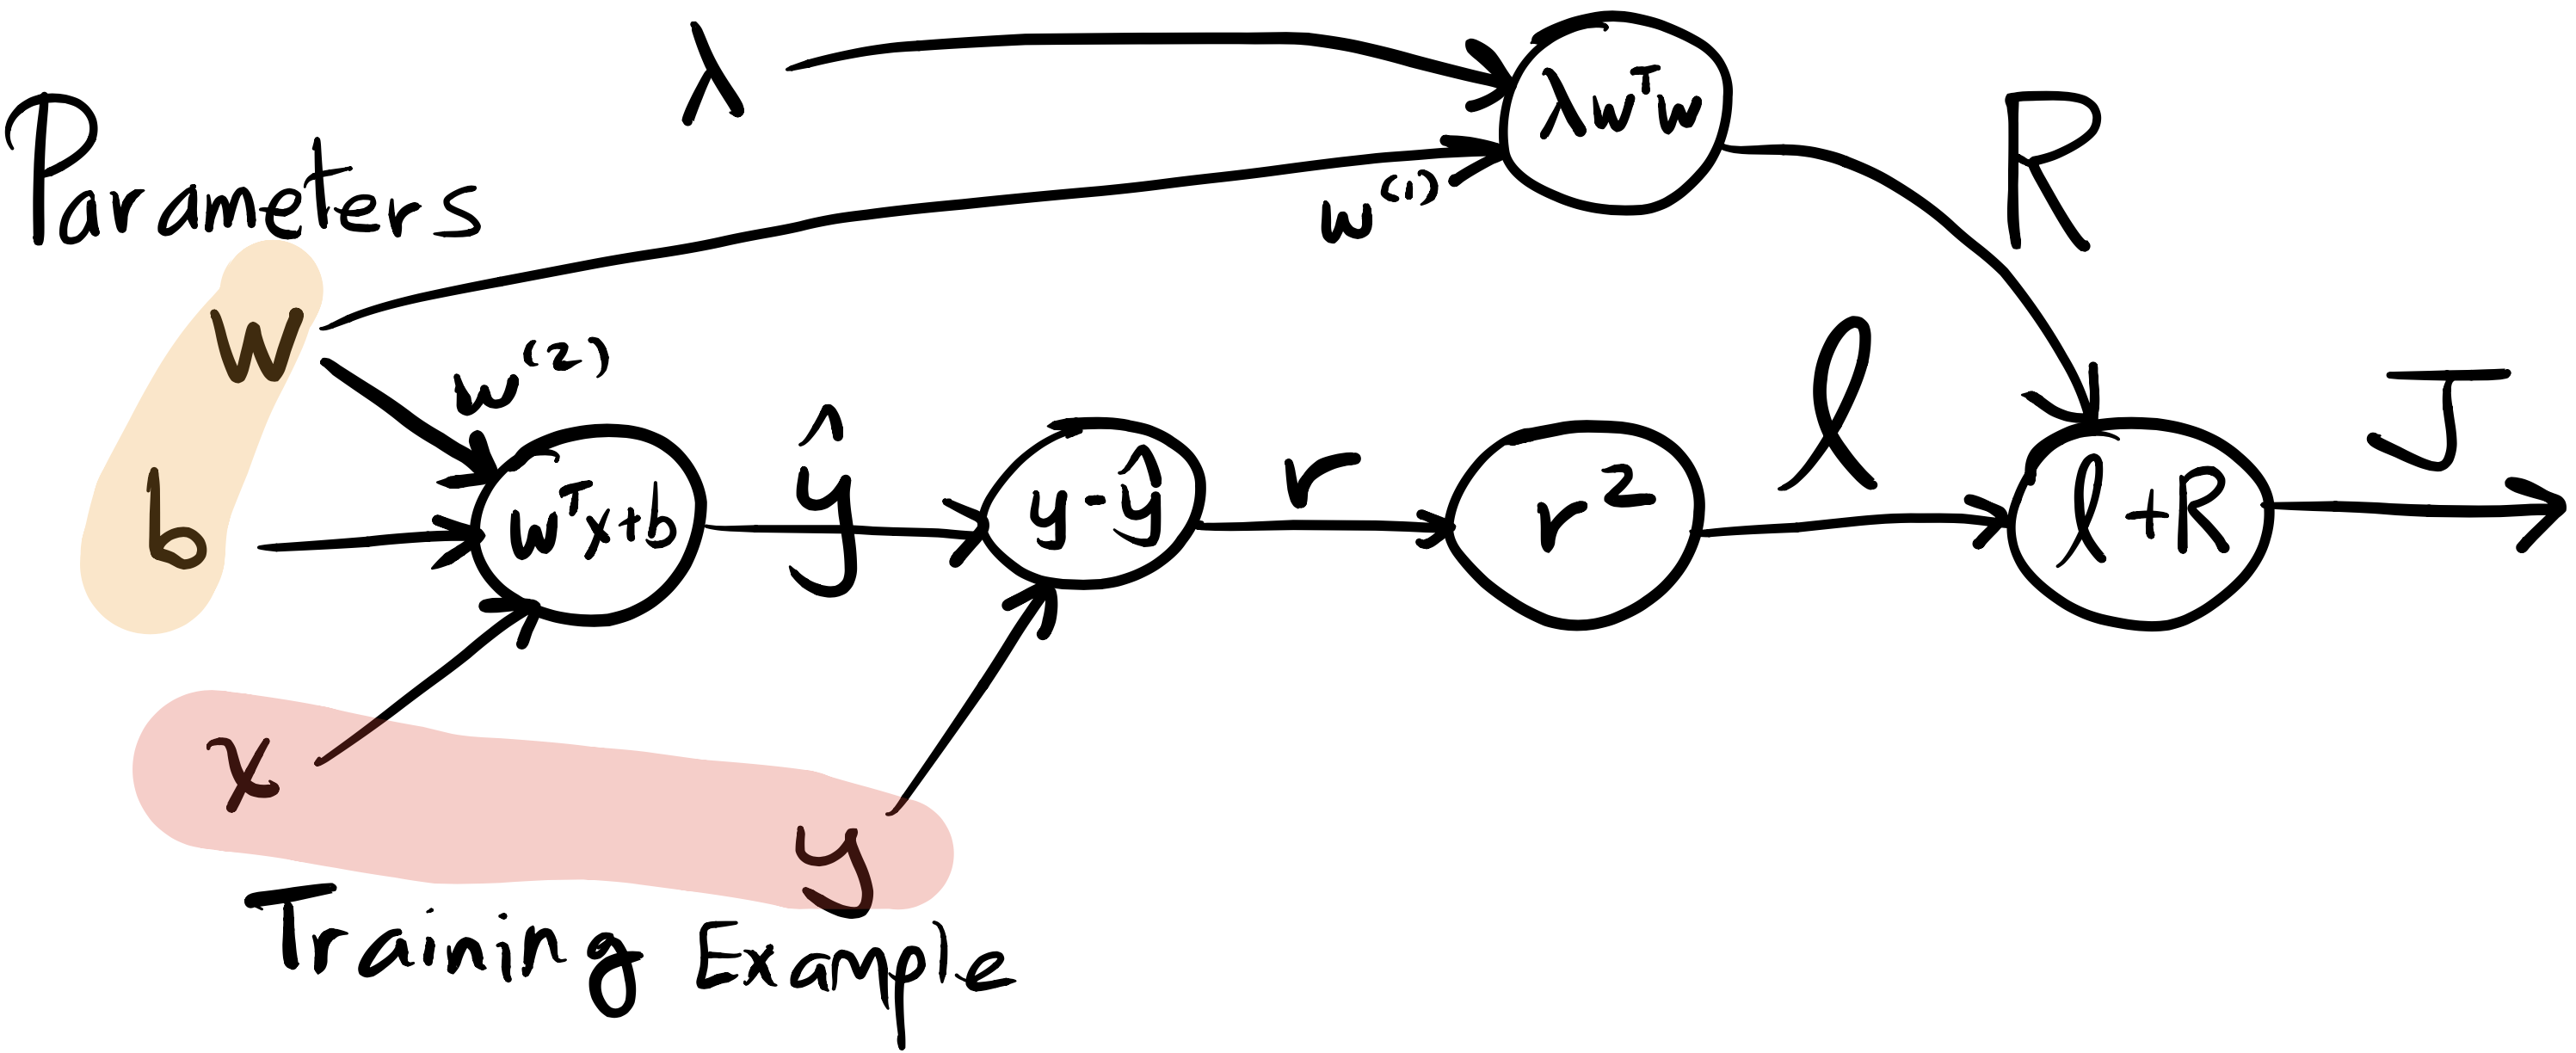
\includegraphics[width=1\columnwidth]{figures/ridge-regression-comp-graph-labels-2copies}
%
%\pause{}
%
%\column{.45\textwidth}
%
%\begin{eqnarray*}
%\frac{\partial J}{\partial\hat{y}} & = & \frac{\partial J}{\partial\ell}\frac{\partial\ell}{\partial r}\frac{\partial r}{\partial\hat{y}}=\left(1\right)(2r)\left(-1\right)=-2r\\
%\frac{\partial J}{\partial w_{j}^{(2)}} & = & \pause\frac{\partial J}{\partial\hat{y}}\frac{\partial\hat{y}}{\partial w_{j}^{(2)}}=\frac{\partial J}{\partial\hat{y}}x_{j}\\
%\frac{\partial J}{\partial w_{j}^{(1)}} & = & \pause\frac{\partial J}{\partial R}\frac{\partial R}{\partial w_{j}^{(1)}}=\left(1\right)\left(2\lambda w_{j}^{(1)}\right)\\
%\frac{\partial J}{\partial w_{j}} & = & \pause\frac{\partial J}{\partial w_{j}^{(1)}}+\frac{\partial J}{\partial w_{j}^{(2)}}
%\end{eqnarray*}
%
%\end{columns}
%
%\end{itemize}
%\end{frame}

\subsection{General Backpropagation}
\begin{frame}
{Backpropagation overview}
\begin{itemize}
\item \textbf{Learning}: run gradient descent to find the parameters that minimize our objective $J$.
\item Backpropagation: compute gradient w.r.t. each (trainable) parameter $\frac{\partial J}{\partial \theta_i}$.
\end{itemize}

\begin{columns}
\begin{column}{0.45\textwidth}
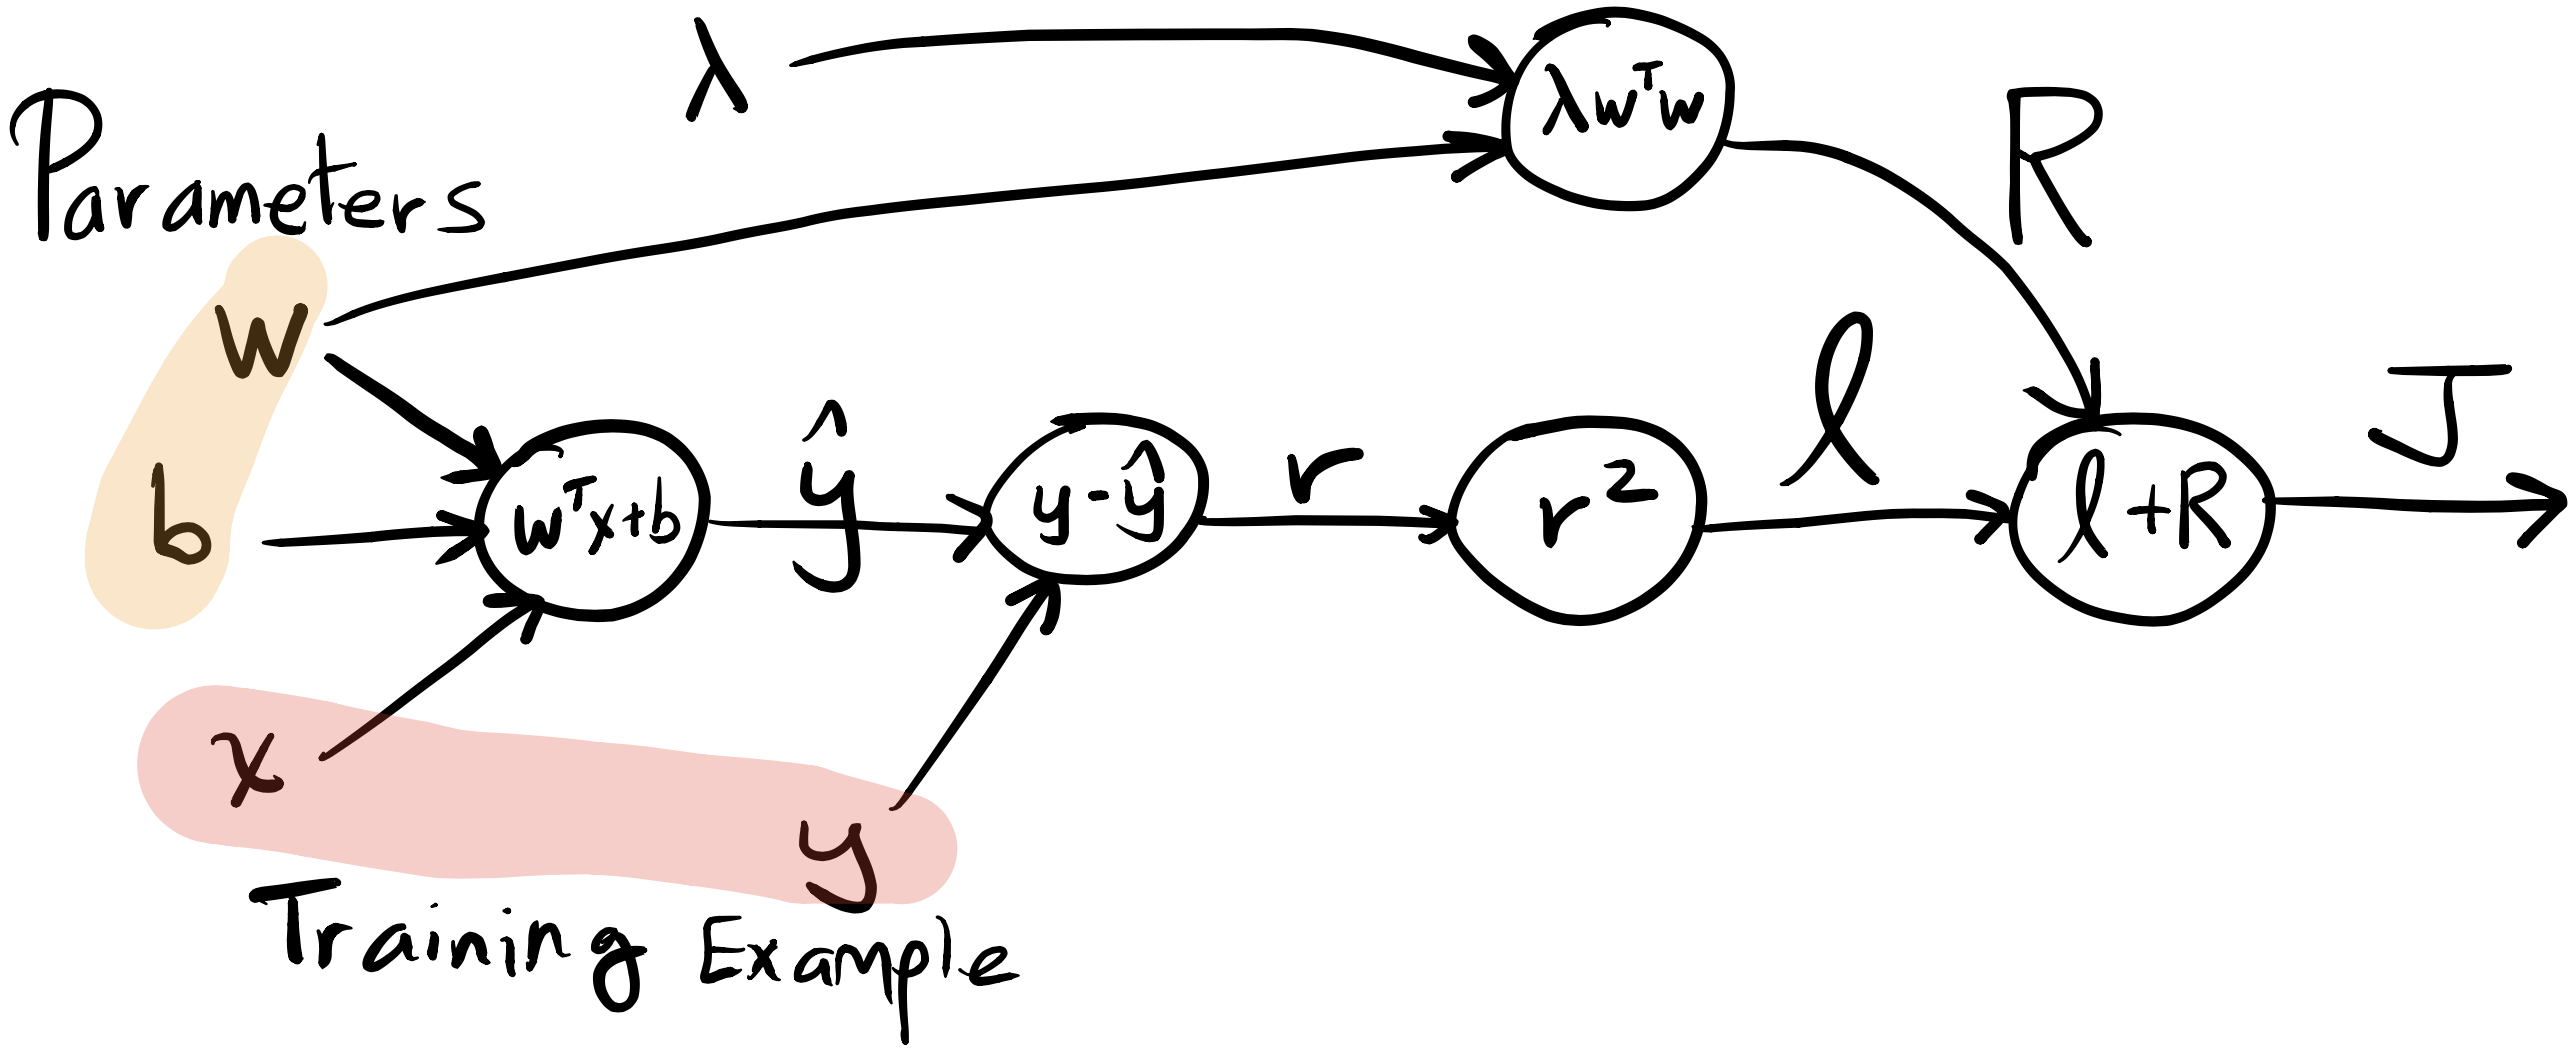
\includegraphics[width=1\columnwidth]{figures/ridge-regression-comp-graph-labels}
\end{column}
\begin{column}{0.55\textwidth}
\begin{description}[Backward pass]
\item[Forward pass] Compute intermediate function values, \ie output of each node
\item[Backward pass] Compute the partial derivative of $J$ w.r.t. all intermediate variables and the model parameters
\end{description}
\begin{simpleblock}{How to save computation?}
\pause
\begin{itemize}
\item Path sharing: each node needs to \emph{cache the intermediate results}.
\item Think dynamic programming.
\end{itemize}
\end{simpleblock}
\end{column}
\end{columns}
\end{frame}

\begin{frame}
{Forward pass}
\begin{itemize}
\item Order nodes by \textbf{topological sort} (every node appears before its children)
\item For each node, compute the output given the input (output of its parents).
\item Forward at intermediate node $f_i$ and $f_j$:
\end{itemize}
\begin{center}
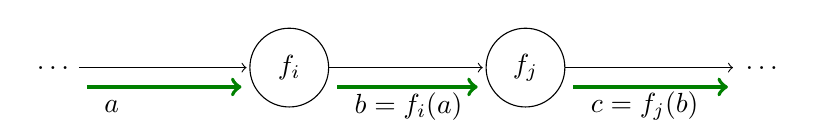
\begin{tikzpicture}[shorten >=1pt]
      	\tikzstyle{unit}=[draw,shape=circle,minimum size =1cm]

		\node (start) at (0,1){$\ldots$};
       	\node[unit](i) at (3,1){$f_i$};
        	\node[unit](j) at (6,1){$f_j$};
        	\node (end) at (9,1){$\ldots$};

        	\draw[->] (i) -- (j);
        	\draw[->] (start) -- (i);
        	\draw[->] (j) -- (end);
		
		\begin{scope}[transform canvas={yshift=-.7em}]
		\draw [->, Green, line width=0.05cm, shorten <=1mm, shorten >=1mm] (start) -- node {} (i);
  		\draw [->, Green, line width=0.05cm, shorten <=1mm, shorten >=1mm] (i) -- node {} (j);
  		\draw [->, Green, line width=0.05cm, shorten <=1mm, shorten >=1mm] (j) -- node {} (end);
		\end{scope}
		
		\begin{scope}[transform canvas={yshift=-1.4em}]
		\node (i-in) [right=0.2cm of start] {$a$};
		\node (j-in) [right=0.2cm of i] {$b=f_i(a)$};
		\node (j-out) [right=0.2cm of j] {$c=f_j(b)$};
		\end{scope}
\end{tikzpicture}
\end{center}
\end{frame}

\begin{frame}
{Backward pass}
\begin{itemize}
\item Order nodes in \textbf{reverse topological order} (every node appear after its children)
\item For each node, compute the partial derivative of its output w.r.t. its input, multiplied by the partial derivative from its children (chain rule).
\item Backward at intermediate node $f_i$:
\end{itemize}
\begin{center}
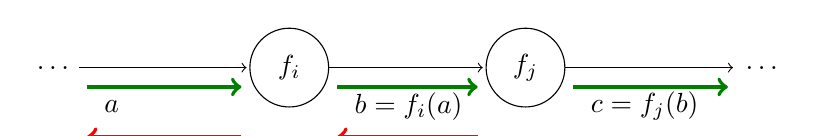
\begin{tikzpicture}[shorten >=1pt]
      	\tikzstyle{unit}=[draw,shape=circle,minimum size =1cm]

		\node (start) at (0,1){$\ldots$};
       	\node[unit](i) at (3,1){$f_i$};
        	\node[unit](j) at (6,1){$f_j$};
        	\node (end) at (9,1){$\ldots$};

        	\draw[->] (i) -- (j);
        	\draw[->] (start) -- (i);
        	\draw[->] (j) -- (end);
		
		\begin{scope}[transform canvas={yshift=-.7em}]
		\draw [->, Green, line width=0.05cm, shorten <=1mm, shorten >=1mm] (start) -- node {} (i);
  		\draw [->, Green, line width=0.05cm, shorten <=1mm, shorten >=1mm] (i) -- node {} (j);
  		\draw [->, Green, line width=0.05cm, shorten <=1mm, shorten >=1mm] (j) -- node {} (end);
		\end{scope}
		
		\begin{scope}[transform canvas={yshift=-1.4em}]
		\node (i-in) [right=0.2cm of start] {$a$};
		\node (j-in) [right=0.2cm of i] {$b=f_i(a)$};
		\node (j-out) [right=0.2cm of j] {$c=f_j(b)$};
		\end{scope}
		
		\begin{scope}[transform canvas={yshift=-2.5em}]
		\draw [<-, red, line width=0.05cm, shorten <=1mm, shorten >=1mm] (start) -- node {} (i);
  		\draw [<-, red, line width=0.05cm, shorten <=1mm, shorten >=1mm] (i) -- node {} (j);
%  		\draw [<-, red, line width=0.05cm, shorten <=1mm, shorten >=1mm] (j) -- node {} (end);
		\end{scope}
		
		\begin{scope}[transform canvas={yshift=-3.4em}]
		\node (i-out) [left=0.2cm of i] {$g_i=g_j \cdot \frac{\partial b}{\partial a} = \frac{\partial J}{\partial a}$};
		\node (j-out) [left=0.2cm of j] {$g_j=\frac{\partial J}{\partial b}$};
		\end{scope}
\end{tikzpicture}
\end{center}
\end{frame}

\begin{frame}{Multiple children}
\begin{itemize}
\item First sum partial derivatives from all children, then multiply.
\begin{columns}[c]

\column{.45\textwidth}

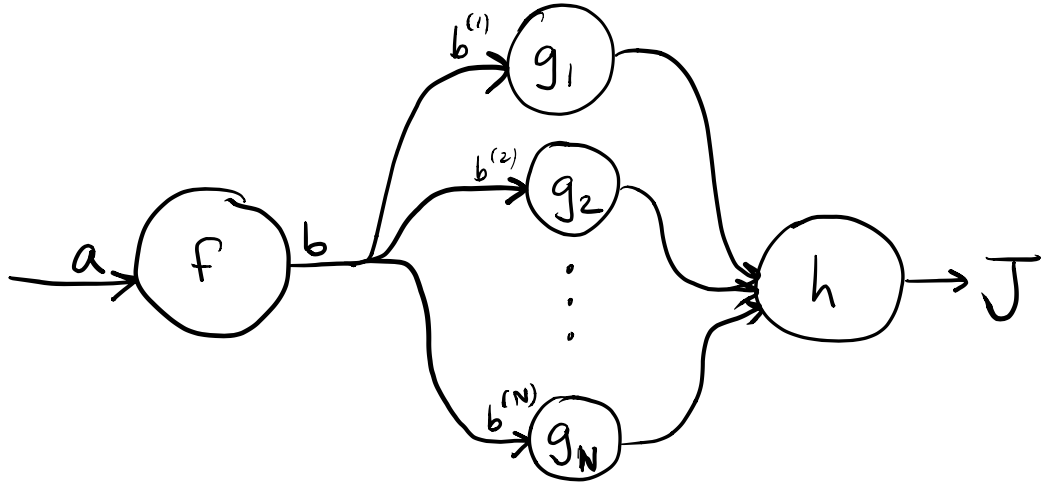
\includegraphics[width=1\columnwidth]{figures/backprop-general-node}

\pause{}

\column{.5\textwidth}
\begin{itemize}
\item Backprop for node $f$:
\item \textbf{Input}: $\frac{\partial J}{\partial b^{(1)}},\ldots,\frac{\partial J}{\partial b^{(N)}}$
\\
(Partials w.r.t. inputs to all children)
\item \textbf{Output}: 
\begin{eqnarray*}
\frac{\partial J}{\partial b} & = & \sum_{k=1}^{N}\frac{\partial J}{\partial b^{(k)}}\\
\text{ }\frac{\partial J}{\partial a} & = & \frac{\partial J}{\partial b}\frac{\partial b}{\partial a}
\end{eqnarray*}
\end{itemize}
\end{columns}

\end{itemize}
\end{frame}
%
%
\begin{frame}
{Backpropagation in practice}
\begin{itemize}
\item Inputs and outputs of nodes are generally \emph{vectorized} (efficient to compute on GPUs).
\item Computation graphs can be composed from a set of \emph{basic operation nodes}, \eg addition/multiplication, dot product, logistic function etc. 
\item Programming paradigms:
\begin{description}[Imperative]
\item[Symbolic] Specify all computation before data---efficient, \eg Tensorflow.
\item[Imperative] Specify the computation step by step---flexible/easier to write, \eg Pytorch.
\item[Hybrid] Can use either paradigm for computation subgraphs, \eg MXNet.  
\end{description}
\end{itemize}
\end{frame}

\begin{frame}
{Non-convex optimization}
\begin{figure}
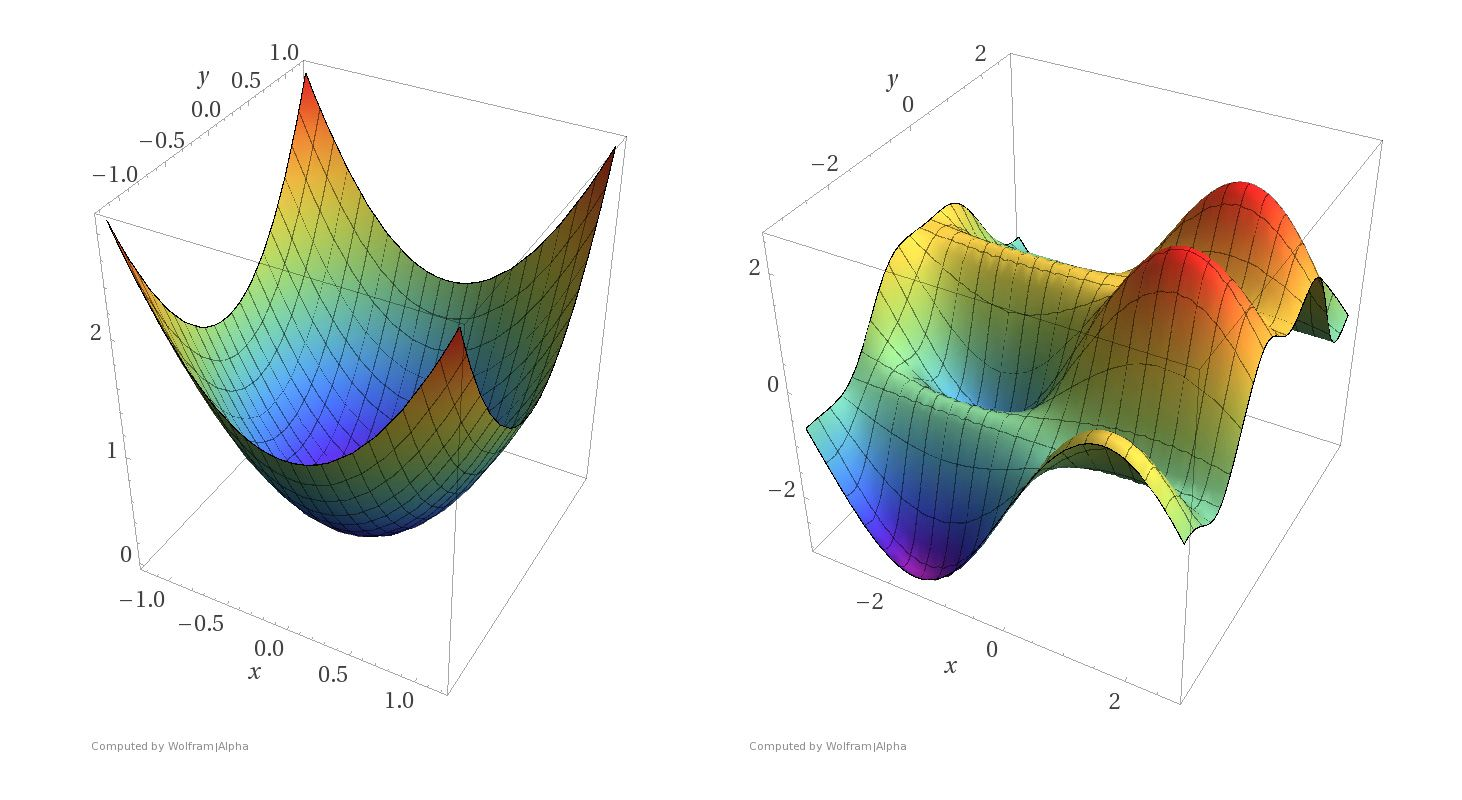
\includegraphics[height=0.7\textheight]{figures/convex_cost_function}
\end{figure}
\begin{itemize}
\item Left: convex loss function. Right: non-convex loss function.
\end{itemize}
\end{frame}

\begin{frame}
{Non-convex optimization: challenges}
\begin{simpleblock}{Optimization of neural networks is generally hard.}
\begin{columns}
\begin{column}{0.6\textwidth}
\begin{itemize}
\item Converge to a bad local minimum.
\begin{itemize}
\item Try different initialization and rerun.
\end{itemize}
\item Saddle point. 
\begin{itemize}
\item Doesn't often happen with SGD. 
\item Second partial derivative test.
\end{itemize}
\item ``Flat'' region: low gradient magnitude
\begin{itemize}
\item Use ReLU instead of sigmoid as activation functions.
\end{itemize}
\item High curvature: high gradient magnitude
\begin{itemize}
\item Gradient clipping.
\item Adaptive step sizes.
\end{itemize}
\end{itemize}
\end{column}
\begin{column}{0.4\textwidth}
\begin{figure}
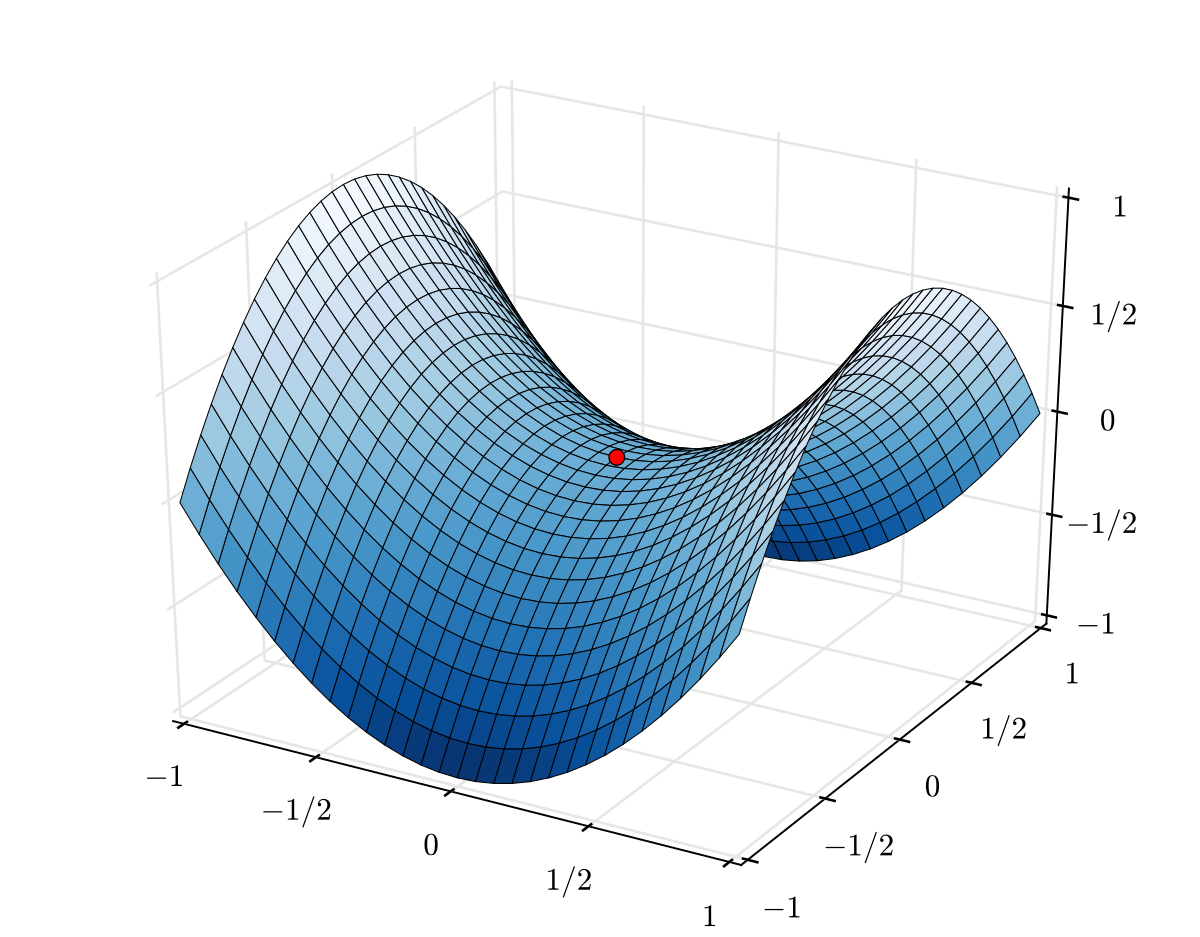
\includegraphics[width=0.8\columnwidth]{figures/saddle_point}
\end{figure}
\end{column}
\end{columns}
\end{simpleblock}
\let\thefootnote\relax\footnotetext{\tiny{Reference: Chris De Sa's slides (CS6787 Lecture 7).}}
\end{frame}

\begin{frame}
{Review}
\begin{itemize}
\item Backpropagation is an algorithm to compute gradient (partial derivatives + chain rule) efficiently.
\item It is used in gradient descent optimization with neural networks.
\item Key idea: function composition and dynamic programming
\item In practice, efficient software exists (backpropagation, neural network building blocks, optimization algorithms etc.).
\end{itemize}
\end{frame}


\end{document}
